% set 0.5 inch indentation
\setlength{\parindent}{0.5in} 
% set paragraph space = 0 space
\setlength{\parskip}{0mm}
% set line space 1.5
\setlength{\baselineskip}{1.6em}

\chapter{METHODOLOGY}
\label{ch:methodology}

The different components of the proposed system and how they work together are described in this chapter.

\section{System Overview}
The system uses multiple drones with PixHawk flight controllers, each paired with an individual companion computer and a ground control station (GCS). The operator sets the origin of the global map and select a region of interest on the GCS using Mapviz, a ROS package. The system creates a grid over the region of interest and calculate paths for the drones. After the expected paths are calculated, the system calibrates the drones by finding an accurate transformation between each drone's local frame of reference and the global frame. To accomplish this, the drones move along a predefined flight path while the transformations between each drone's local map and the global map is refined. After calibration is complete, the system coordinates the flights of the drones as they move along the paths the system calculated, ensuring coverage of the region of interest. While flying their paths, the drones stream images from their cameras to the GCS. On the GCS, the SfM module receives the images and constructs an aerial map (a textured 3D mesh) with respect to the global map frame for the region of interest initially selected by the operator.


All the components runs on a single computer while simulating the system. In simulation mode, PX4 will be run in software in the loop (SITL) mode. Gazebo will be used to visualize the physical world and render simulated video feeds. Network Simulator 3 (NS3) will be used to simulate the networking functions of the wireless mesh network.

\section{System Design}

The different components comprising the system are described here.

\subsection{Components}

The system can be divided into two domains, one comprising the components in the drones, and the other comprising the components in the GCS. Components running on drones do not share information with other drones; they only share with the GCS. These components will be involved with vehicle platform manipulation and forwarding the images captured. The components on the GCS will be involved with getting the initial region of interest from the operator, planning the path of each drone, coordinating the movement of each drone during plan execution, requesting and receiving images from the drones, and aerial mapping from the images received.

The flight controller is installed with PX4 firmware. The companion computers and the GCS runs Ubuntu or Raspbian Linux with the Robot Operating System (ROS) installed and is connected to a wireless mesh network through IEEE 802.11 devices.

The components on the GCS are illustrated in Figure~\ref{fig:gcs-components} and as follows:
\begin{itemize}
	\item \textit{Computer.} An i7 laptop with 16 GB of RAM running Ubuntu 18 is the processing unit of the GCS.
	\item \textit{Wirless mesh router.}  Wireless mesh router provides mesh network to the laptop, as well as maintain mesh network with the drones.
	\item \textit{Robot Operating System.} All the components is designed and implemented with ROS as the base infrastructure. This gives access to the plethora of ROS tools and packages.
	\item \textit{mapviz.} Mapviz running as a plugin inside rqt is the GUI interface for the system. Mapviz is a ROS-based visualization tool with a plug-in system focused on visualization of 2D data. It shows tiled maps using the Microsoft Bing Maps API and has plugins to select polygons on the map, show markers, show NavSat data, among other features that fit the requirements of this system. Mapviz also allows us to fix the origin of the global map.
	\item \textit{image\_pipeline}. ROS image pipeline is used to rectify the image obtained from the cameras attached to the drones.
	\item \textit{pegasus\_planner.} A new multi-agent path planning ROS node designed for the project.
	\item \textit{pegasus\_controller.} A new ROS node that calculates and maintains translations between different map frames, monitor links with the drones, transmit path planning information to the drones, and coordinate the drones during flight.
	\item \textit{pegasus\_image\_subscriber.} A new ROS node that requests and receives images from the drones.
	\item \textit{pegasus\_image\_rectify.} A new ROS node that rectifies the received images for each individual drones' cameras using image\_pipeline.  
	\item \textit{Structure from Motion software.} An aerial map is constructed using the rectified images acquired from drones by this component. ODM (Open Drone Map) is used to build the map. ODM uses OpenSfM, an open source SfM software framework.
\end{itemize}

\begin{figure}
	\centering
	\caption[Pegasus system overview]{\small Architecture diagram of ground control station.}
	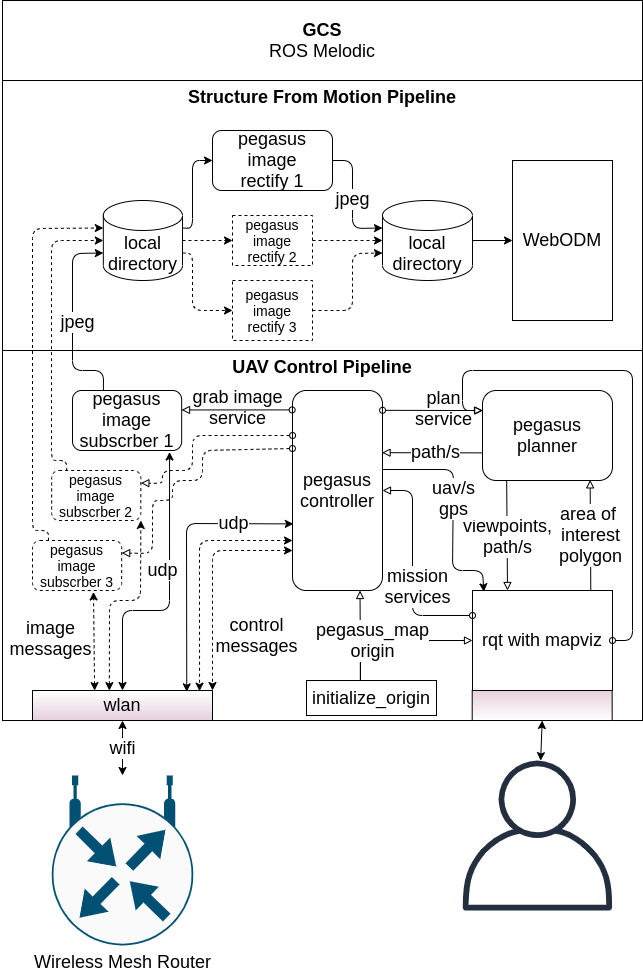
\includegraphics[width=5in]{figures/methodology/methodology-gcs-components}
	\label{fig:gcs-components}
\end{figure}

The components in the drones are illustrated in Figure~\ref{fig:drone-components} and as follows:
\begin{itemize}
	\item \textit{Flight Controller.} The drones will use Pixhawk flight controllers with PX4 as their firmware.
	\item \textit{Companion Computer.} The companion computer will control the flight controller in OFFBOARD mode through a serial link.
	\item \textit{Mobile wireless mesh router.} The mobile wireless mesh router will maintain mesh network using OSLR, and will provide network to the companion computer through ethernet link.
	\item \textit{USB camera.} The USB camera attached to the computer will enable the drone to capture images.
	\item \textit{Robot Operating System.} The software components will be designed and implemented as ROS nodes.
	\item \textit{mavros.} The companion computer will use mavros, a ROS package for MavLink communication between companion computers, and flight controllers, to control the flight controller in OFFBOARD.
	\item \textit{gscam.}  Gscam will be used to acquire video stream from the camera attached to the drone. Gscam is a ROS package which is based upon gstreamer.
	\item \textit{pegasus\_commander.} A new ROS node designed for the project that receives paths and control messages from the GCS. It will publish and subscribe to mavros for controlling, and receiving status of the drone. It will also send to the GCS, the drone's local poses, GPS positions, flight controller status updates, and GCS link monitoring information.
	\item \textit{pegasus\_image\_publisher.} The video feed from the onboard camera will be captured, geo-tagged with GPS information and sent to the GCS by this component.
\end{itemize}

\begin{figure}
	\centering
	\caption[Pegasus GCS system overview]{\small Architecture diagram of drone.}
	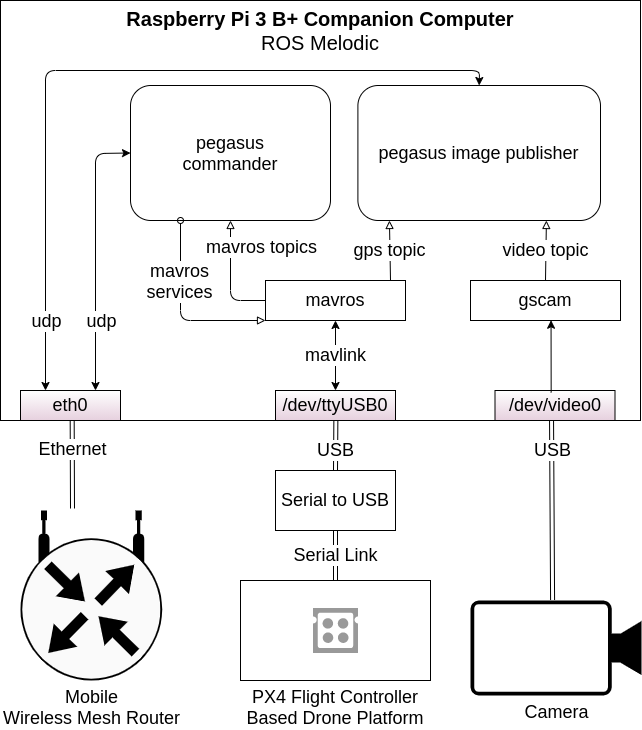
\includegraphics[width=5in]{figures/methodology/methodology-drone-components}
	\label{fig:drone-components}
\end{figure}


The operator will select the global map origin and region of interest through mapviz. The pegasus\_planner will create a grid-based representation of the region of interest and plan the paths for the drones in the global map reference frame.  The path planned by pegasus\_planner will be sent to pegasus\_controller. Pegasus\_controller will run a calibration routine on each of the drones to find the transformation between the local origin of the drone and the global map origin. These transformations allow the system to maintain the global map (pegasus\_map), where planning is carried out and the local map (uav0\_map, uav1\_map, etc.), where the control of the drones are achieved as shown in Figure~\ref{fig:map-heirarichy}. After calibration completes, pegasus\_controller will transform the paths for the drones from global map to the local map for each drone and send it to the drone. Pegasus\_controller will monitor the link with each drone by sending a periodic heart-beat packet. If a drone does not receive a heart-beat packet for some interval, it will change to Return To Home (RTL) mode and abort its current path. To avoid collision, pegasus\_controller will also maintain a path index counter. Paths are made up of a list of poses. Pegasus\_controller will tell each drone to move to the next pose in its path when all the drones have reached their current goal pose.

\begin{figure}
	\centering
	\caption[Different maps in pegasus system.]{\small Different maps in pegasus system.}
	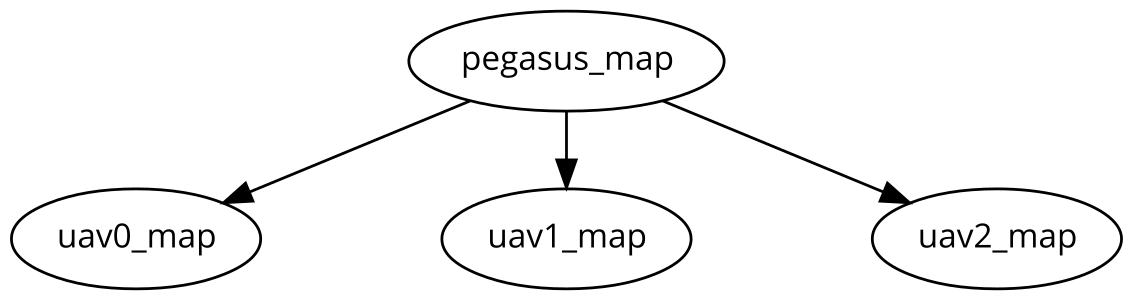
\includegraphics[width=5in]{figures/methodology/map-transformation-heirarichy}
	\label{fig:map-heirarichy}
\end{figure}


The drones will use mavros, which exposes MavLink protocol parameters and services as ROS topics and services. Pegasus\_commander will receive commands and path information from the GCS and execute its plan while sending local poses, global GPS positions, and flight controller state information back to the GCS. Gscam will publish video stream from the USB camera as a ROS camera topic. The pegasus\_image\_publisher will capture images from the published camera topic, apply GPS exif tag and send them to the GCS, as it receives request from pegasus\_image\_subscriber that will save the received images to a local directory. 

Pegasus\_rectify\_image will rectify the images using the camera calibration parameters, prepare the images for map building and save them to a directory in GCS . The SfM module will construct an aerial map for the region of interest selected by the operator from these images.


\subsection{Simulation}

Most of the components will remain the same regardless of whether running in simulation or in the real world. The simulation will run in a single computer. Four more components will be utilized to simulate the system:
\begin{itemize}
	\item \textit{Gazebo.} Gazebo simulator will be used because it supports fleet of drones and camera feed.
	\item \textit{PX4 Software in the loop.} PX4 firmware will be run as software in the loop, to simulate the drone's firmware. 
	\item \textit{pegasus-net-sim.} A custom network simulator 3 module that will simulate the mobility of the drones and push and pop actual control messages and video feed between the drones and the GCS through the simulator. It will also publish the SNR status of each device in the network.
	\item \textit{pegasus\_network\_status\_util\_node.} A custom ROS node that will receive noise and signal strength from pegasus-net-sim and publish the signal-to-noise ratio (SNR) value of each drone as ROS topic.
\end{itemize}


PX4 software in the loop (SITL) will be used to simulate the drone. PX4 SITL uses Gazebo to simulate the world, the drone mechanics and the video feed. Pegasus-net-sim, a Network Simulator 3 custom module will be used to simulate the wireless mesh network. Pegasus-net-sim will receive the model info from Gazebo and update the position of its nodes. Each node in pegasus-net-sim will have NS3PegasusApp, a custom NS3 application installed, which will send and receive packets in the simulated network. Pegasus-net-sim will function as a proxy application that will receive data in one UDP port, simulate it in NS3 and transmit it through another UDP socket. Using the trace feature in NS3, pegasus-net-sim will publish the noise and signal value for each node of the wireless mesh network.

Figure~\ref{fig:gcs-components-simulated} and Figure~\ref{fig:drone-components-simulated} illustrates the components used in simulation. 

\begin{figure}
	\centering
	\caption[Pegasus system simulaion overview]{\small Architecture diagram of simulated ground control station.}
	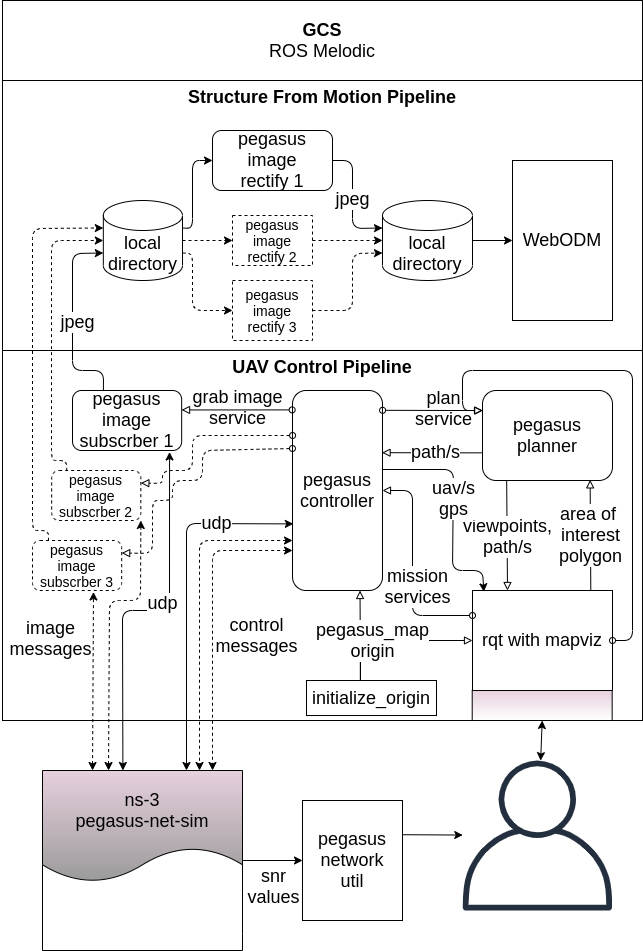
\includegraphics[width=5in]{figures/methodology/methodology-gcs-components-simulated}
	\label{fig:gcs-components-simulated}
\end{figure}
\begin{figure}
	\centering
	\caption[Pegasus GCS system simulation overview]{\small Architecture diagram of simulated drone.}
	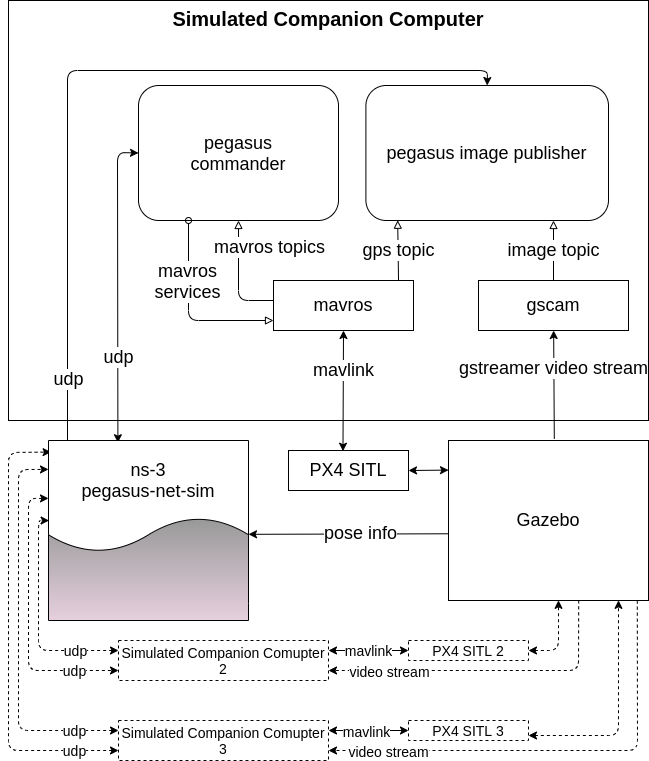
\includegraphics[width=5in]{figures/methodology/methodology-drone-components-simulated}
	\label{fig:drone-components-simulated}
\end{figure}


\subsubsection{pegasus-net-sim}

Network Simulator 3 is used to simulate wireless mesh network infrastructure. ns3 provides a framework to write simulations that can be integrated with other software. For this study ns3 should be able to:
\begin{itemize}
	\item Simulate a wireless mesh network with OLSR as the underlying mesh protocol to build the routing table for each node.
	\item Update the position of the nodes using the pose information from Gazebo. Gazebo library will be used to subscribe to gazebo pose topic.
	\item Inject and eject real world traffic between GCS and drones to the ns3 simulation. \texttt{pegasus-net-sim} will be designed as a proxy application between the components of the pegasus system to intercept traffic between them.
	\item Trace the signal noise value different nodes and publish it using the trace feature of ns3.
\end{itemize}

The architecture diagram of pegasus-net-sim is given in Figure~\ref{fig:pegasus-net-sim}. NS3PegasusDroneApp is a custom application for ns3 that will inject and eject the udp packets to and from the simulation. Each ns3 node will have a NS3PegasusDroneApp installed. A NS3PegasusDroneApp will have a set of PegassUDPSocket encapsulating real udp sockets and its virtual ns3 socket counterpart. Each PegasusUDPSocket class will have transmit and receive threads. These threads will continuously poll for any packet to send or receive in the real udp socket. PegasusUDPSocket will have a tx and rx lockless queue. Receive thread of a socket will write to the rx queue when it receives a packet. Transmit thread will poll the tx queue and transmit the packet to socket. NS3PegasusDroneApp running in ns3 simulation will poll the rx/tx queues of the PegasusUDPSocket in its set and inject/eject the packets to its virtual udp socket inside the simulation.

\begin{figure}
	\centering
	\caption[Architecture of \texttt{pegasus-net-sim}]{\small Architecture diagram of \texttt{pegasus-net-sim}.}
	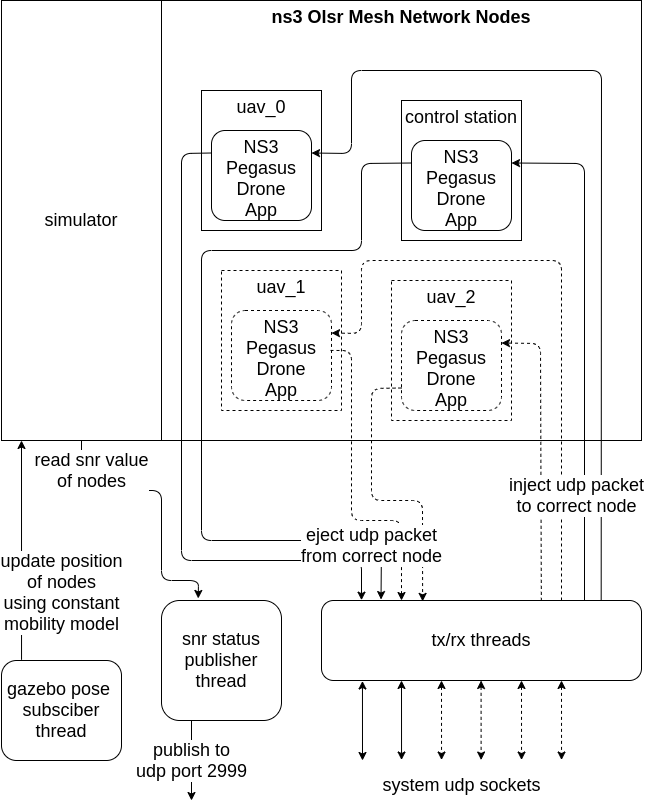
\includegraphics[width=5in]{figures/methodology/methodology-pegasus-net-sim}
	\label{fig:pegasus-net-sim}
\end{figure}

\begin{figure} 
	\centering
	\caption[Example of \texttt{pegasus-net-sim} intercepting packets.]{\small 
		A scenario with one GCS and two drone (a) Communication without network simulation (b) Communication packets being routed through \texttt{pegasus-net-sim}.}
	\subfloat[]{%
		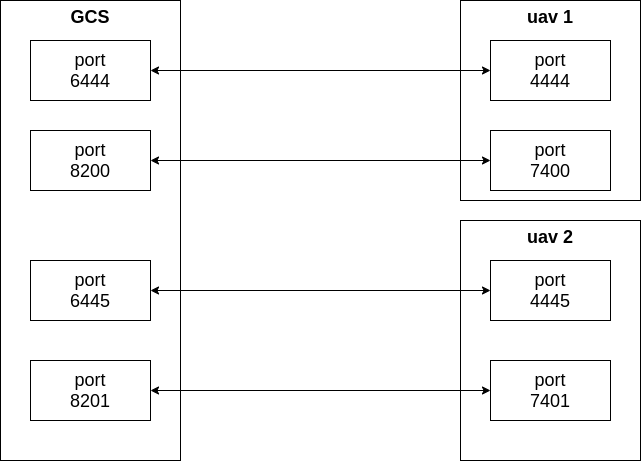
\includegraphics[width=5in]{figures/methodology/methodology-pegasus-net-sim-socket-binding}
	}
	
	\subfloat[]{%
		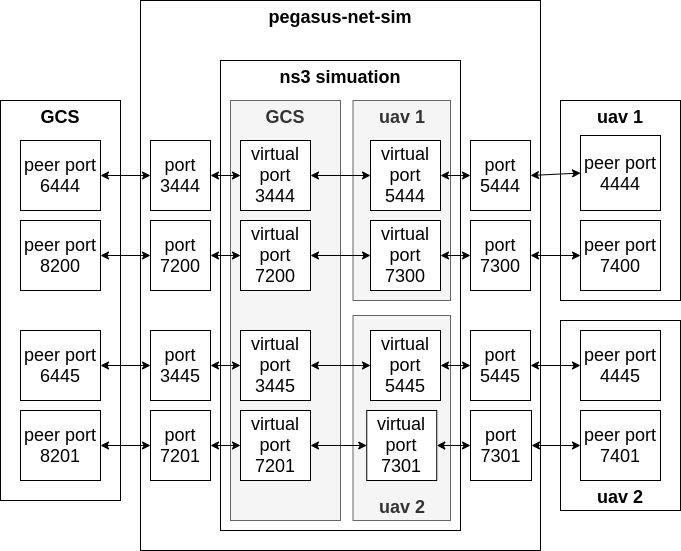
\includegraphics[width=5in]{figures/methodology/methodology-net-sim-routing}
	}
	\label{fig:pegasus-net-sim-simulation-example}
\end{figure}

To intercept and route a packet within pegasus-net-sim, it will have:
\begin{itemize}
	\item \textit{port.} The real udp port which will intercept real world traffic.
	\item \textit{virtual port.} The ns3 virtual port that will simulate port.
	\item \textit{peer port.} The real udp port which the port will transmit to.
	\item \textit{virtual peer port.} The ns3 virtual udp port that the traffic will get transmitted to.
\end{itemize}


Port and virtual port will have the exact same port number. For the configuration, three elements are defined in the tuple \{port, peer port, virtual peer port\}. For the scenario given in Figure~\ref{fig:pegasus-net-sim-simulation-example}, the corresponding configuration in PegasusConfig.cc will be:

\begin{verbatim}

std::map<std::string, std::vector<PegasusPortConfig>> 
PegasusConfig::m_config {
{
"iris_0", {
{5444, 4444, 3444},
{7300, 7400, 7200},
}
},
{
"iris_1", {
{5445, 4445, 3445},
{7301, 7401, 7201},
}
},
{
CONTROL_STATION_STR , {
{3444, 6444, 5444},
{7200, 8200, 7300},
{3445, 6445, 5445},
{7201, 8201, 7301},
}
},
};
\end{verbatim}

\subsection{pegasus\_network\_status\_util\_node}

The ns3 module pegasus-net-sim traces the signal and noise decibel of each packet of each node, smooths and averages it out per 100 millisecond per node and advertises it to udp port 2999. The pegasus\_network\_status\_util\_node reads the information on udp port 2999, and publishes signal to noise ratio (SNR) as ROS topics for each node for the user to analyses. 

\section{Functional Components}
The functional software components of the pegasus system can be categorized as:
\begin{itemize}
	\item \textit{Presentation.} This layer defines how the operator interacts with the system. Solely in the GCS.
	\item \textit{Planning.} This layer will calculate a list of grid based viewpoints and provide path through those viewpoints for the drones in the system, to cover the region of interest selected in the presentation layer. This layer will be in the GCS. 
	\item \textit{Motion control.} This layer will calculate the drones' local and global map transformations and control the motion of the drones according to path calculated in the planning layer. It will also align the drones in a particular direction at the viewpoints where it needs to capture an image and will request image acquisition service to acquire the image. This layer will be in the GCS as well as the drone.
	\item \textit{Image acquisition.}  This layer will be present in the GCS and the drone. It will provide service to capture image from the drone, apply GPS tags and deliver it to the GCS over the network. The images acquired will be saved in a local directory of the GCS.
	\item \textit{Map building.} After the drones have covered their paths, the map building layer will process the images in the local directory of the GCS.
\end{itemize}

\subsection{Presentation}

This layer presents how an end user will interact with the system. The front-end of the system will utilize a ROS package called mapviz. Mapviz will be used as a plugin inside ROS rqt. The ROS rqt will provide a dashboard for the operator to interact with. The GUI that the operator will be presented with is illustrated in Figure~\ref{fig:mapviz-screenshot}. The presentation layer will run in the GCS.

\begin{figure}
	\centering
	\caption[Pegasus presentation dashboard]{\small ROS rqt with mapviz visualizer. Origin for pegasus\_map is set near CSIM.}
	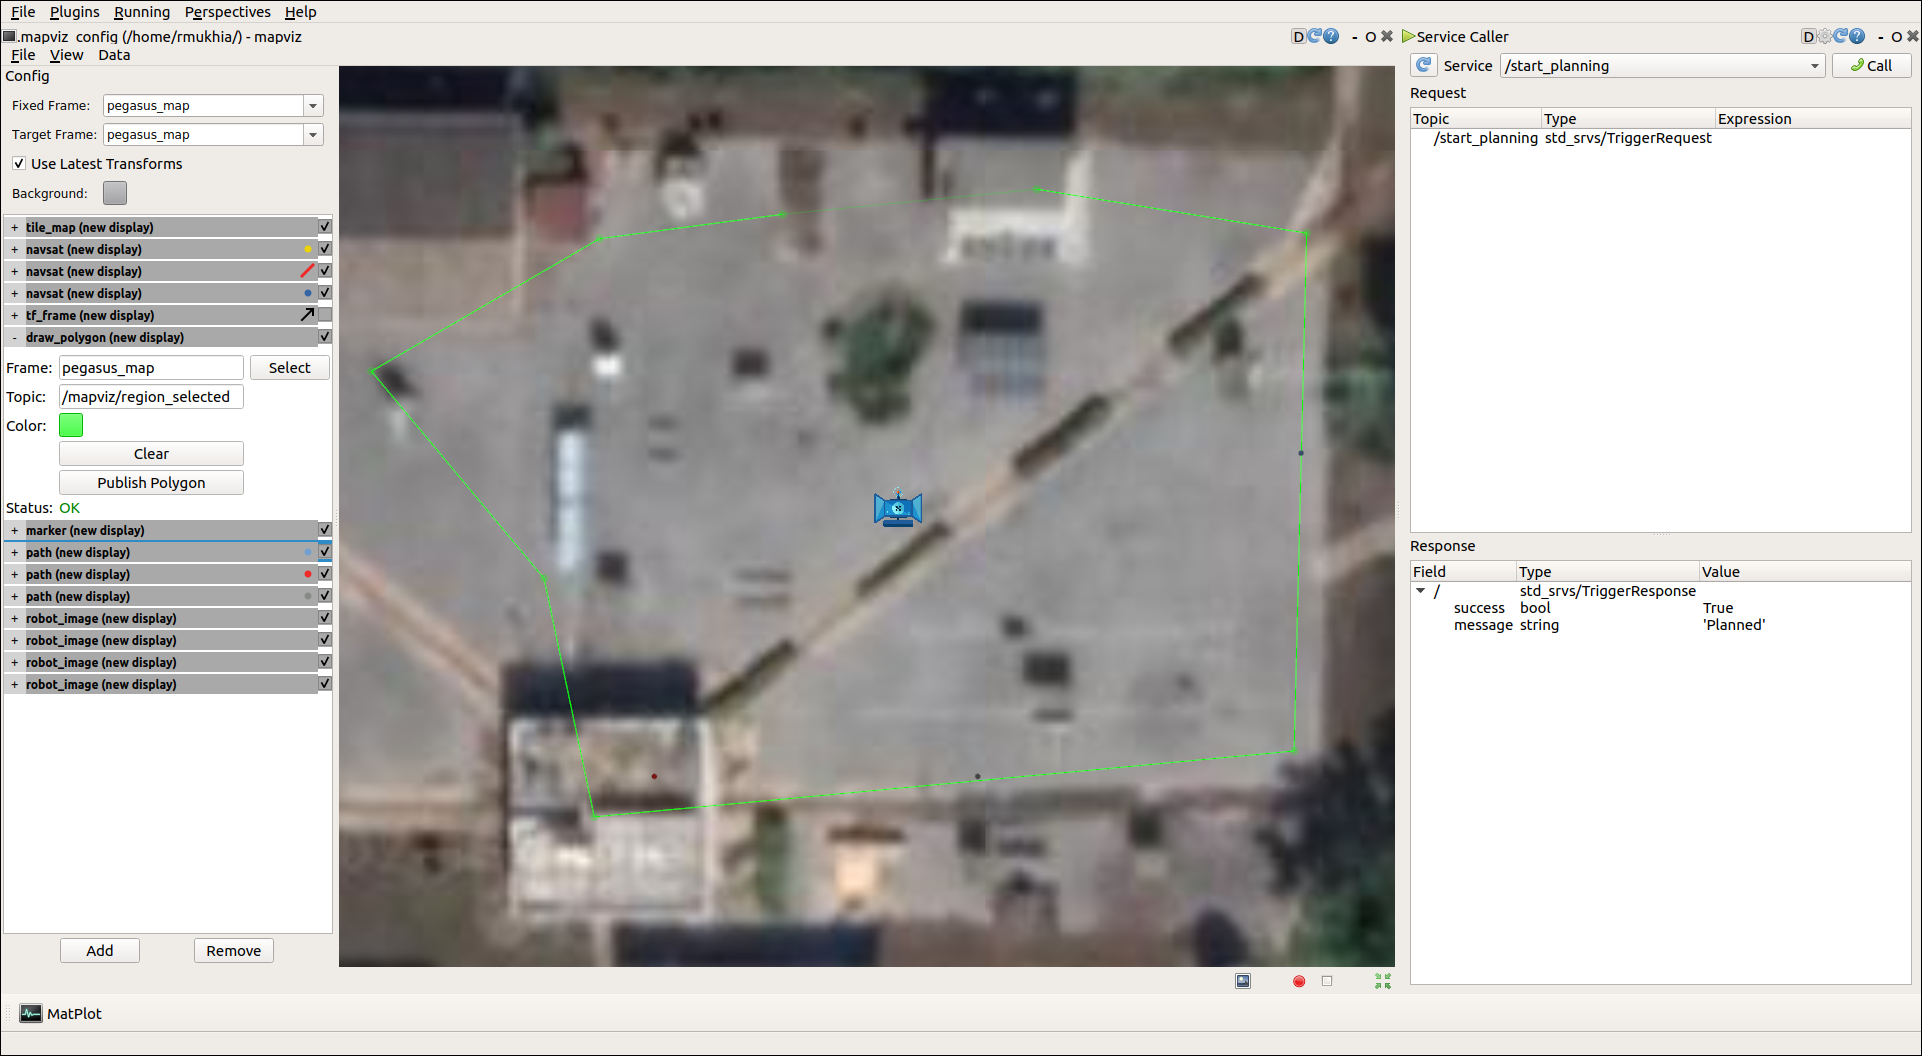
\includegraphics[width=5in]{figures/methodology/presentation/mapviz-1}
	\label{fig:mapviz-screenshot}
\end{figure}


\subsubsection{Mapviz}
Mapviz requires the operator to select the global map origin as a ROS parameter. ROS parameters can be set through the rosparams command-line tool, programmatically or in the launch file. In our case, we set the local map origin though the launch file using the ROS package swri\_transform\_util.


\begin{verbatim}
<?xml version="1.0"?>
<launch>
<node pkg="swri_transform_util" type="initialize_origin.py"
name="initialize_origin" >
<param name="local_xy_frame" value="/pegasus_map"/>
<param name="local_xy_origin" value="control_station"/>
<rosparam param="local_xy_origins">
[{ name: control_station,
latitude: 14.081104,
longitude: 100.612743,
altitude: 7,
heading: 0.0}]
</rosparam>
</node>
<node name = "pegasus_dashboard" pkg = "rqt_gui" type = "rqt_gui" 
respawn = "false" output = "screen" args = 
"--perspective-file $(find pegasus_ros)/pegasus_ros.perspective"/>
</launch>
\end{verbatim}


It will publish two ROS topics:
\begin{itemize}
	\item /local\_xy\_origin: Origin of the global map.
	\item /mapviz/region\_selected: The points of the polygon as selected by the user.
\end{itemize}

The mapviz module can use online map APIs such as google maps and bing maps. For offline use, mapproxy can be used to cache data locally and serve it to mapviz. \textit{https://github.com/danielsnider/MapViz-Tile-Map-Google-Maps-Satellite} provides a docker image for mapproxy that integrates well with mapviz.

The flow that the operator has to follow while using this GUI is presented in Figure~\ref{fig:presentation-flow}.

\begin{figure}
	\centering
	\caption[Operator interaction with pegasus system]{\small A flowchart of the operator's interaction with the presentation layer.}
	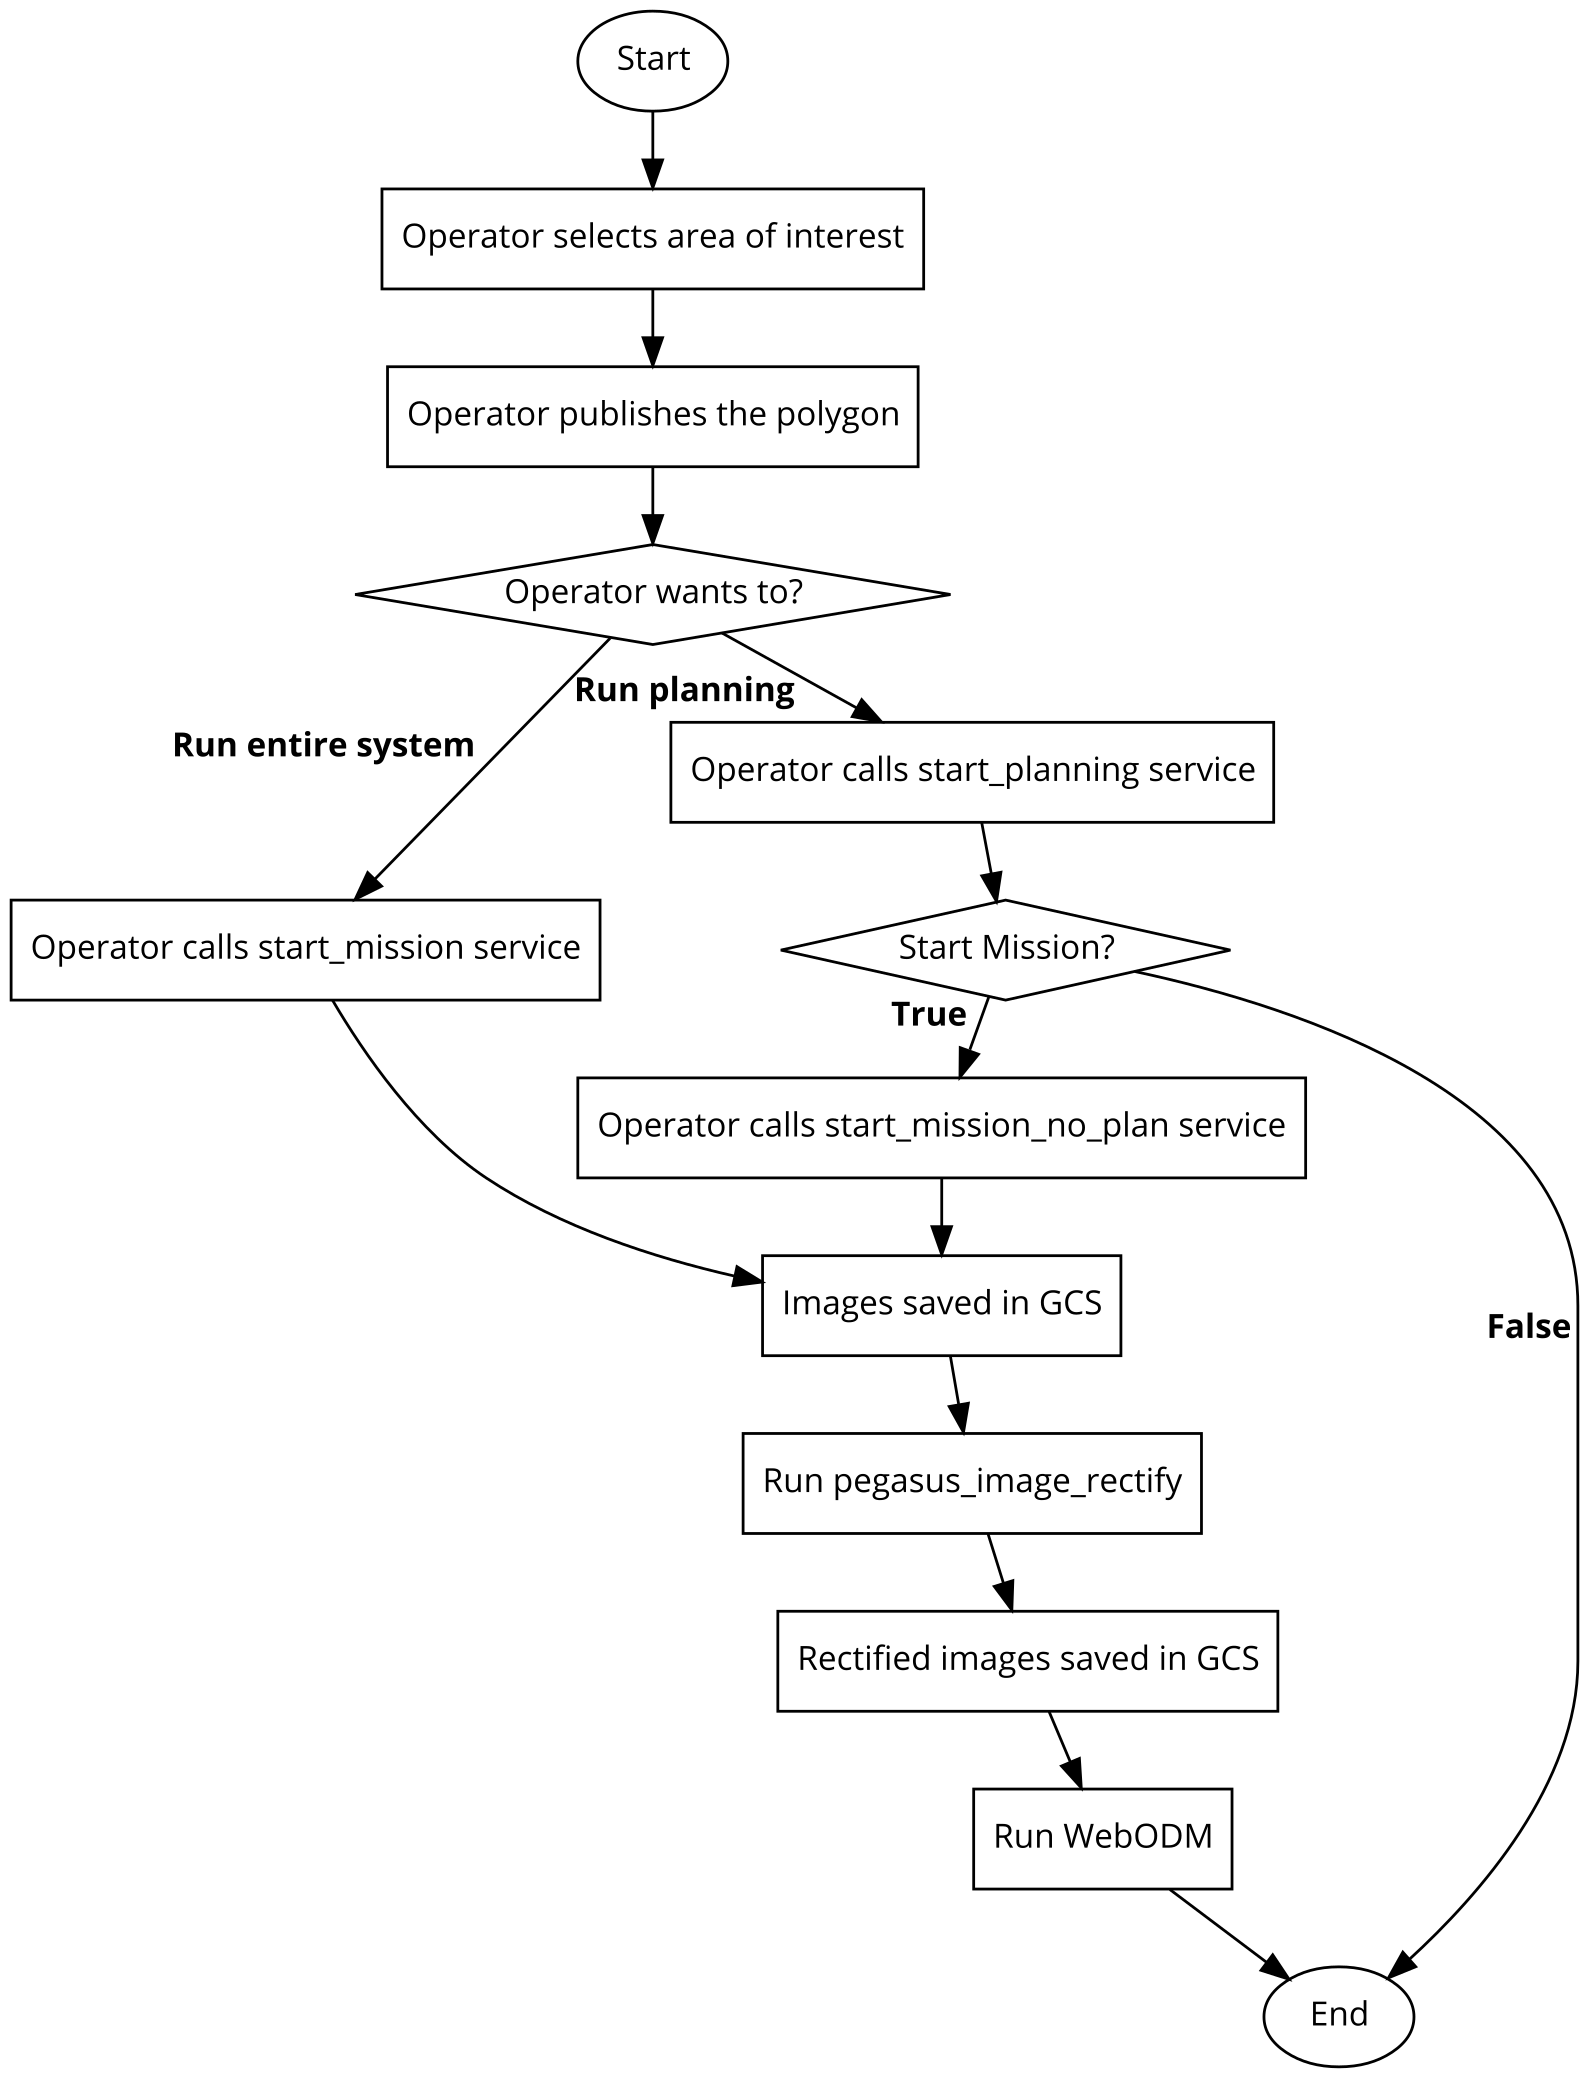
\includegraphics[width=5in]{figures/methodology/presentation/presentation-flow}
	\label{fig:presentation-flow}
\end{figure}


\begin{figure}
	\centering
	\caption[Operator interaction with pegasus system; a scenerio.]{\small 
		A scenario where an operator (a) Selects an area of interest (b) Publishes the polygon (c) Calls start\_planning service.}
	\subfloat[]{%
		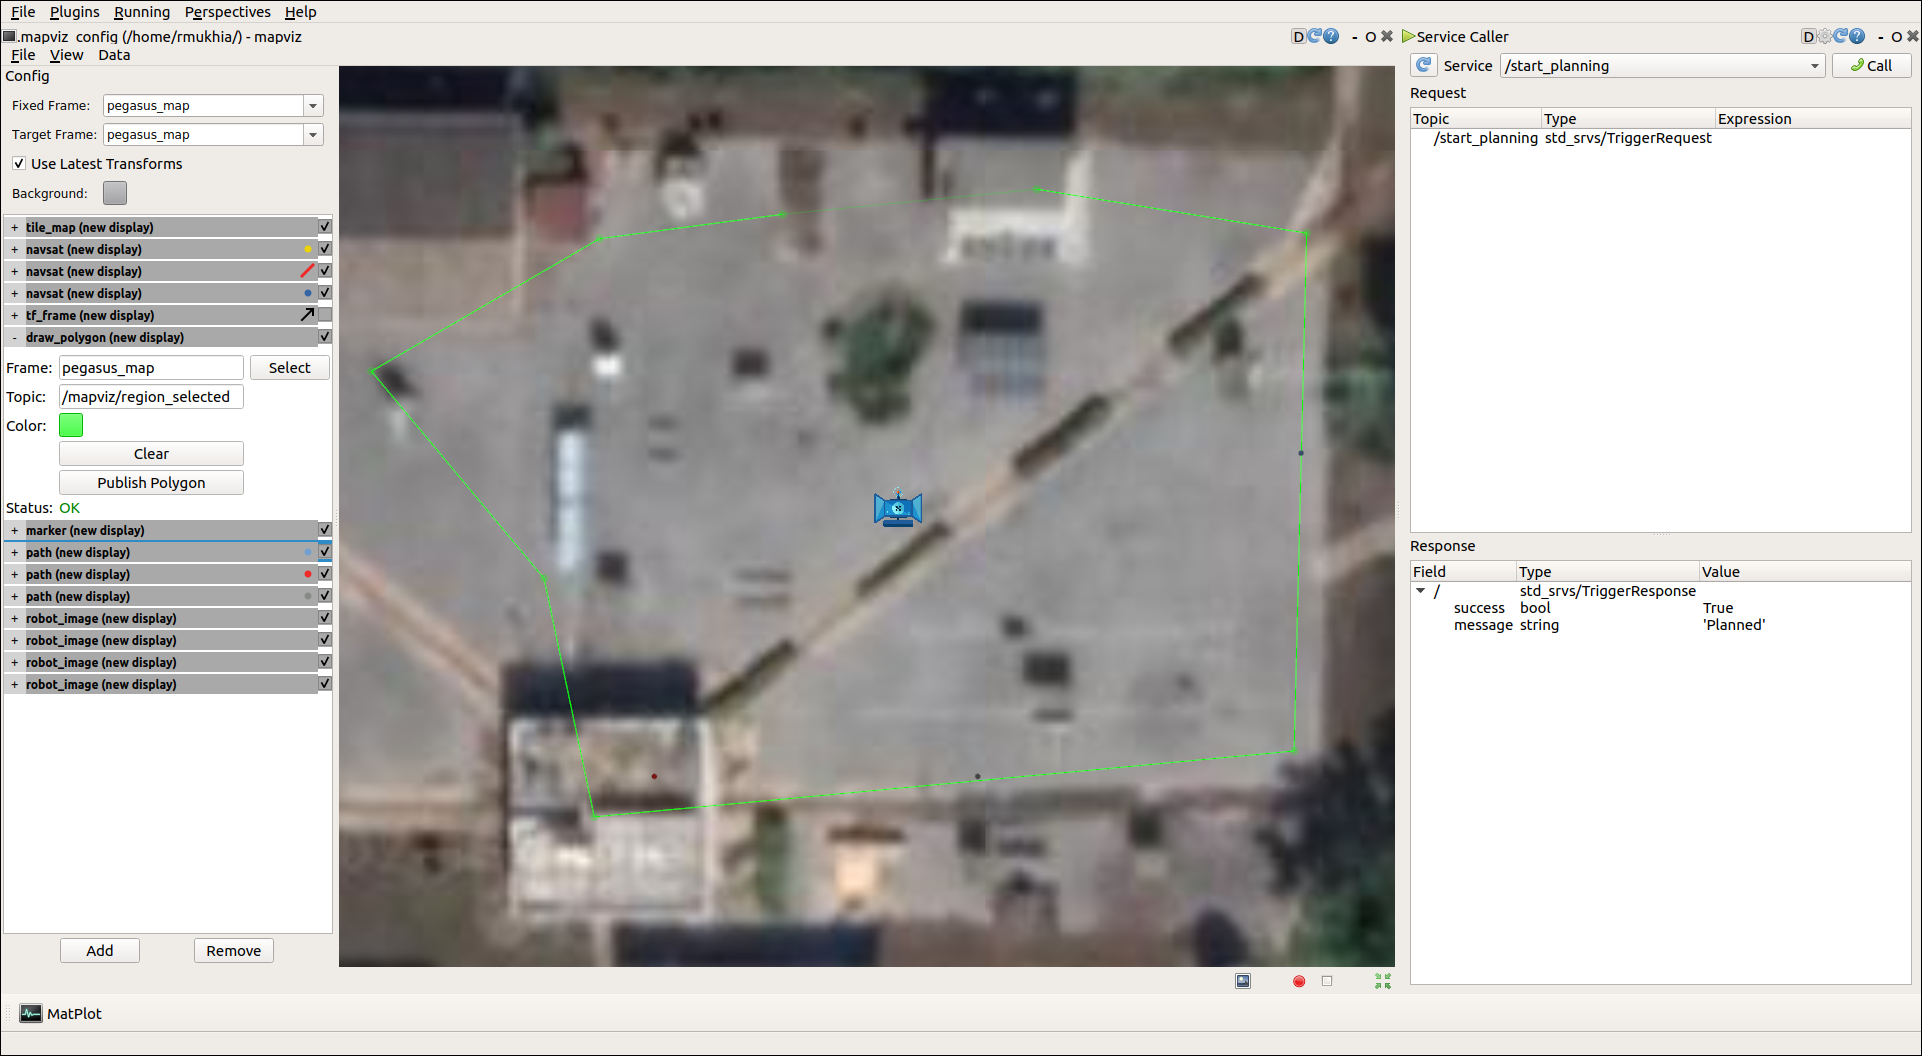
\includegraphics[width=4in]{figures/methodology/presentation/mapviz-1}%
	}
	
	
	\subfloat[]{%
		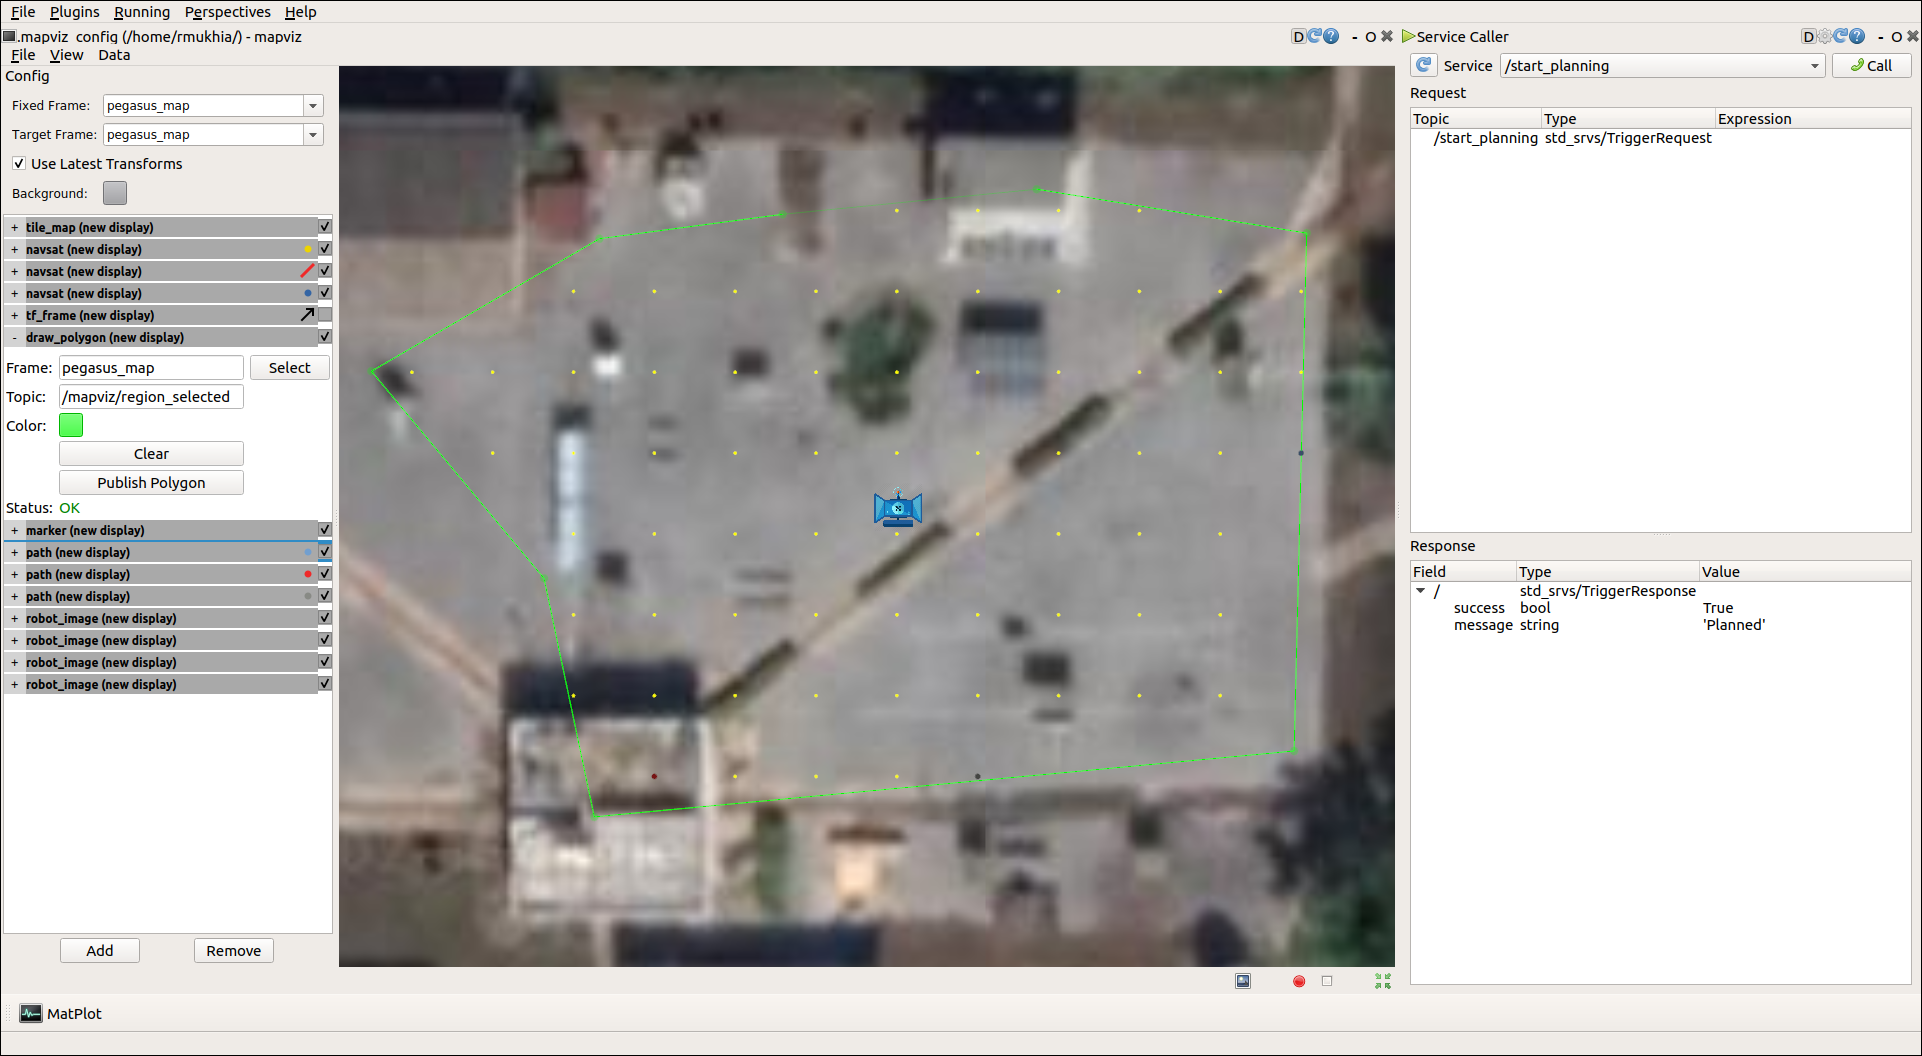
\includegraphics[width=4in]{figures/methodology/presentation/mapviz-2}
	}
	
	
	\subfloat[]{%
		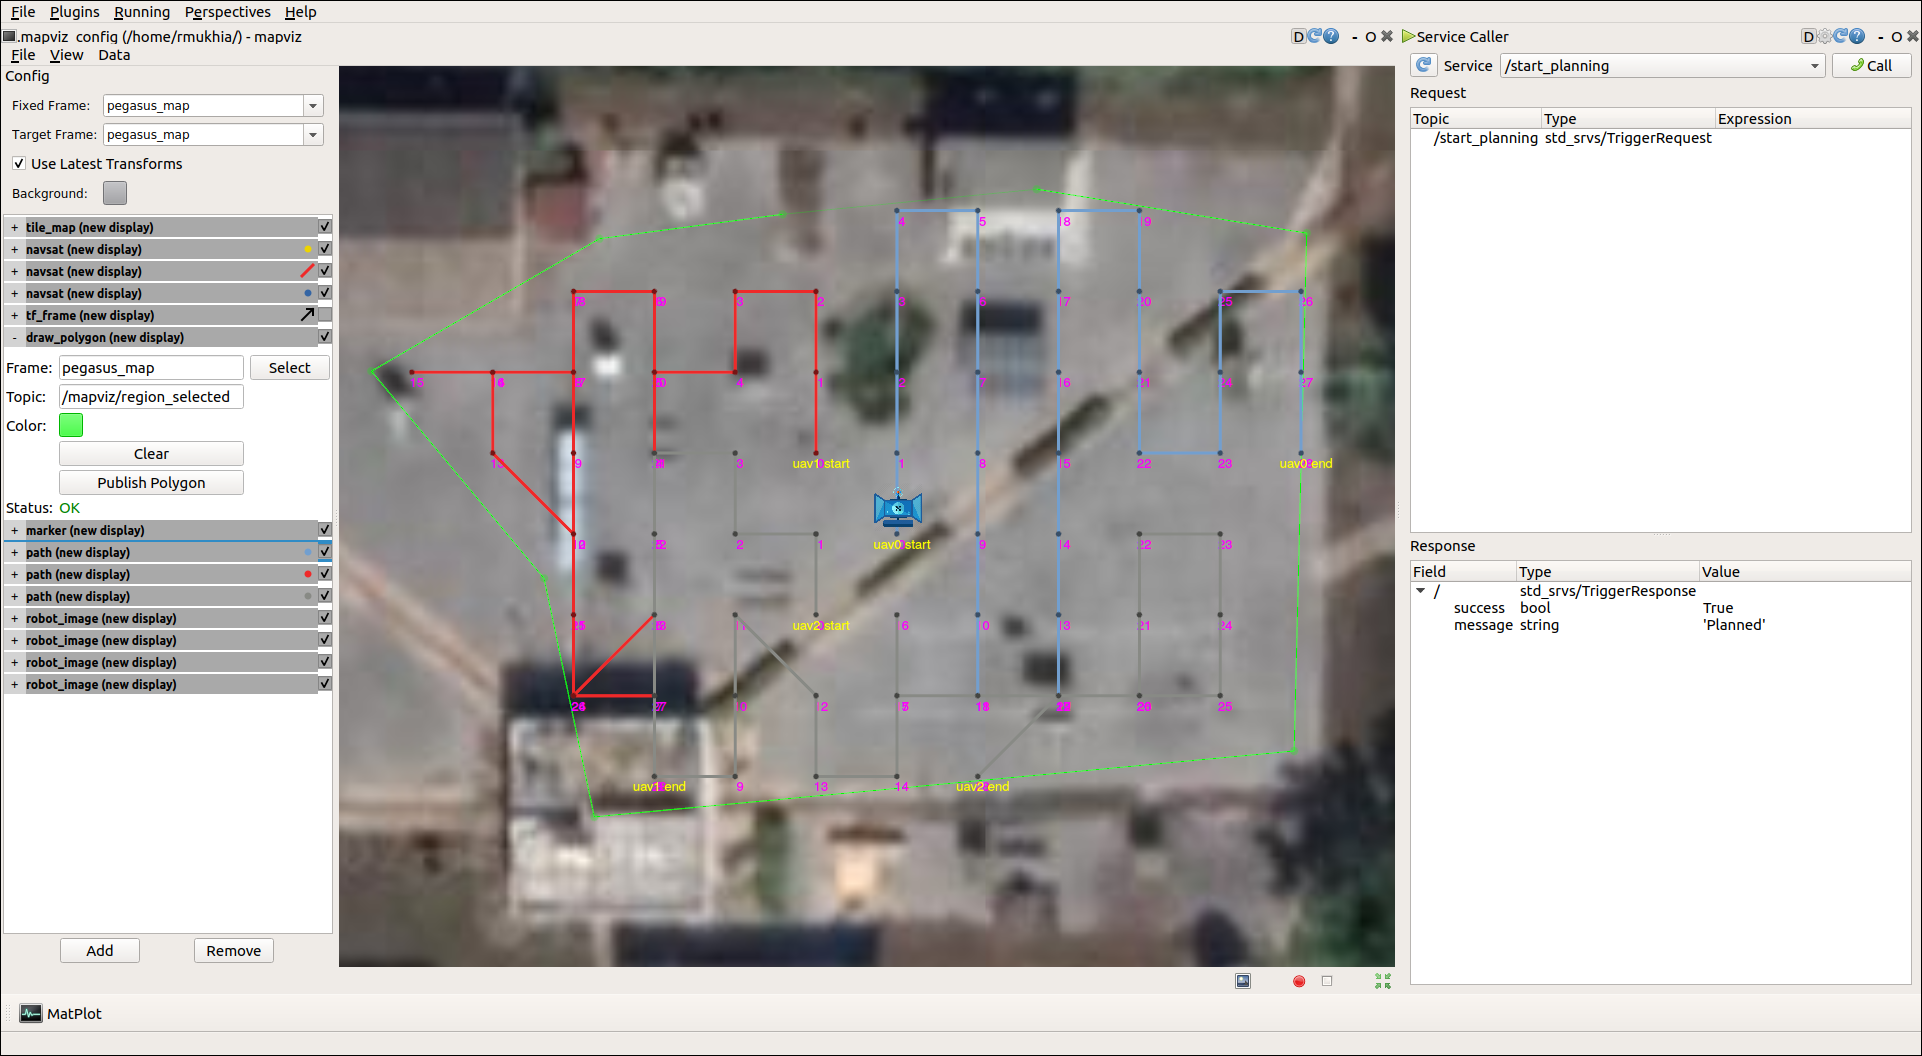
\includegraphics[width=4in]{figures/methodology/presentation/mapviz-3}
	}
	
	\label{fig:presentation-scenerio-1}
\end{figure}


\subsection{Planning}

This layer will compute the path for the drones which will cover the region of interest selected by the operator. It has one component, the pegasus\_planner.

\subsubsection{Pegasus\_planner}

Pegasus\_planner will handle the following tasks:
\begin{itemize}
	\item \textit{Viewpoint generation. } Generate grid cells based viewpoint in the region of interest.
	\item \textit{Multi-agent coverage path planning. } A* search to calculate the optimal paths for each drone, such that they avoid collisions and stay within the constraints of the wireless mesh network in the global map frame.
\end{itemize}

\textbf{Viewpoint Generation}

To generate a valid grid inside the region of interest, consider a polygon with $n$ vertices:

\begin{figure}
	\centering
	\caption[Structure of control messages.]{\small 
		The steps in viewpoint generation (a) Polygon showing the area of interest. (b) Bounding box on the Polygon showing the area of interest. (c) Bottom left position of the cells in the bounding box. (d) Rays projecting from cell centre to $x_{max} + 1$. (e)  Grid cells inside the region of interest. }
	\subfloat[]{%
		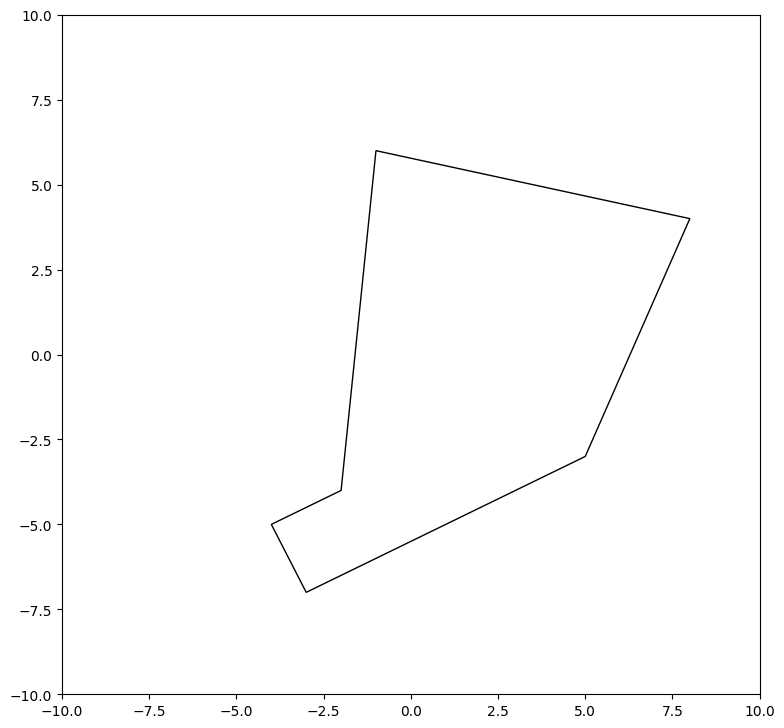
\includegraphics[width=.4\textwidth]{figures/methodology/pegasus_planner/generate_grid/polygon}%
	}
	\subfloat[]{%
		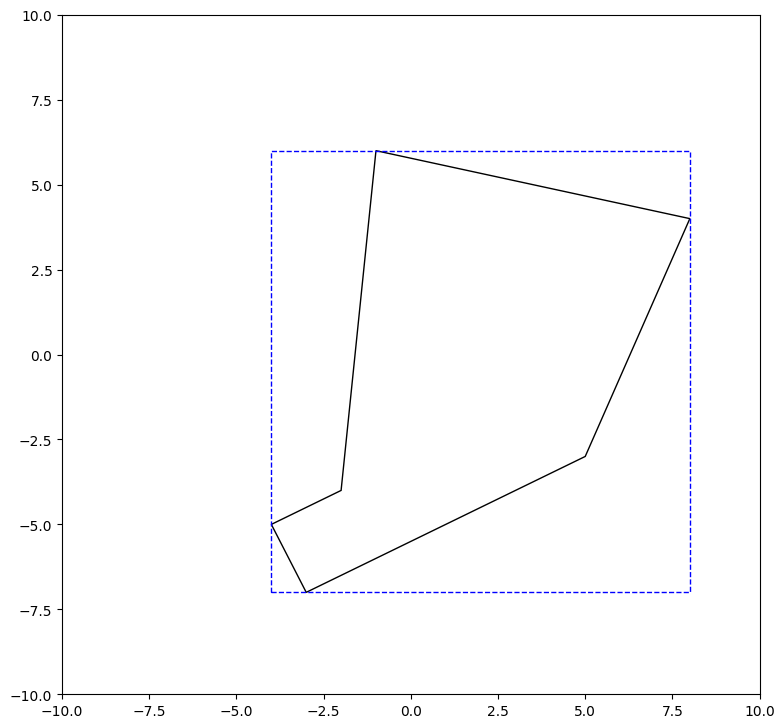
\includegraphics[width=.4\textwidth]{figures/methodology/pegasus_planner/generate_grid/bounding-box}
	}
	
	
	\subfloat[]{%
		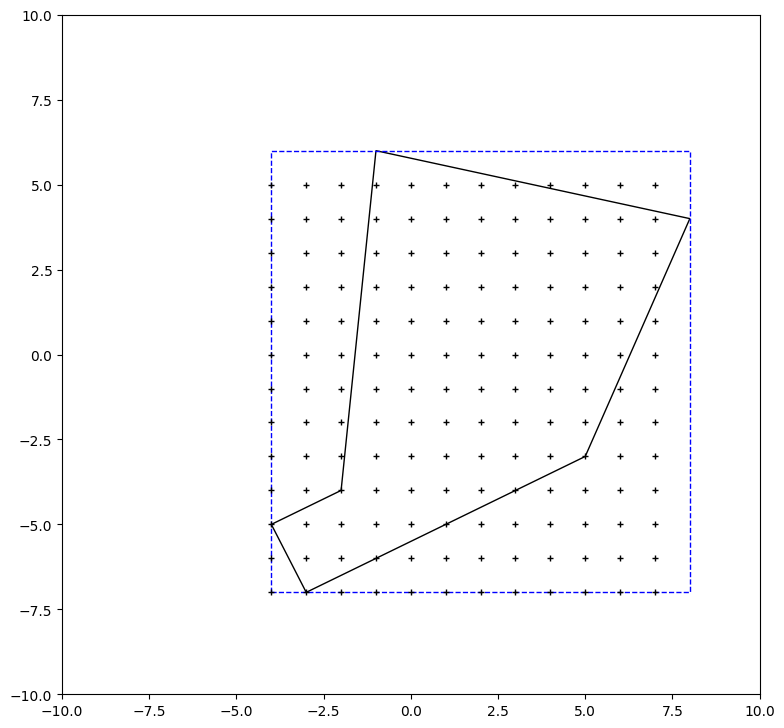
\includegraphics[width=.4\textwidth]{figures/methodology/pegasus_planner/generate_grid/cells}%
	}
	\subfloat[]{%
		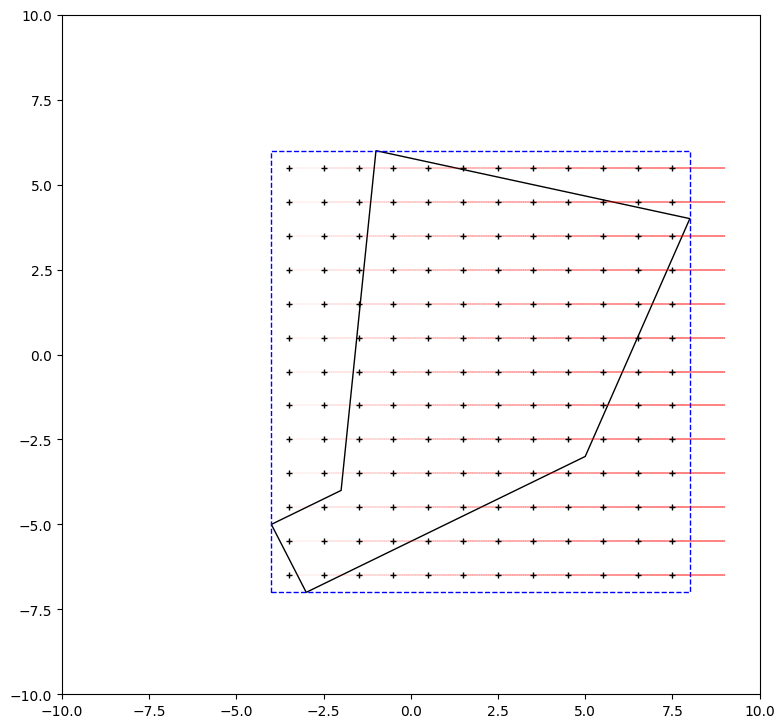
\includegraphics[width=.4\textwidth]{figures/methodology/pegasus_planner/generate_grid/ray}
	}
	
	\subfloat[]{%
		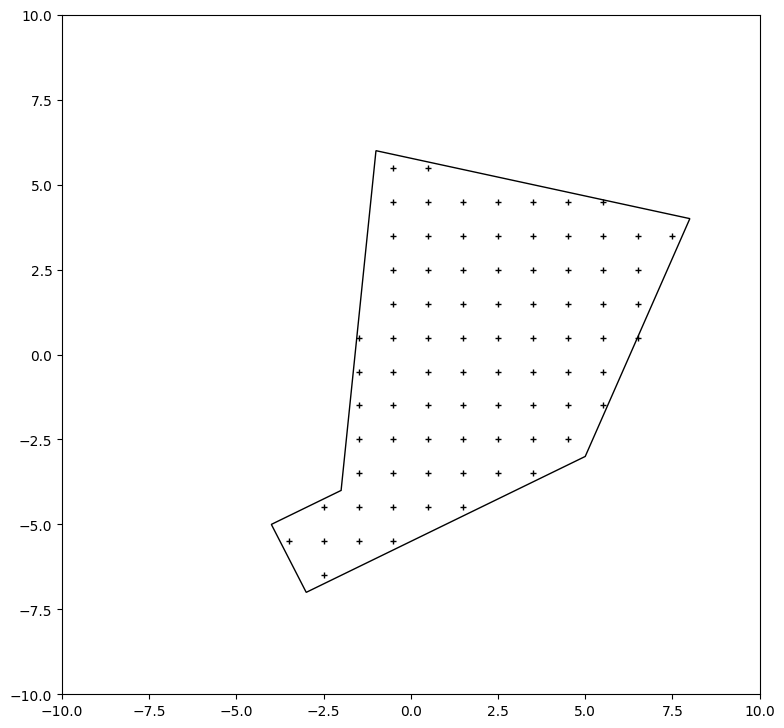
\includegraphics[width=.4\textwidth]{figures/methodology/pegasus_planner/generate_grid/valid-cells}
	}
	
	\label{fig:viewpoint-generation}
\end{figure}

$$
\text{polygon} = \begin{bmatrix}
x^0 & y^0 \\
x^1 & y^1 \\
x^3 & y^2 \\
\vdots  & \vdots \\
x^{n-1} & y^{n-1} \\
\end{bmatrix}. 
$$

The vertices are arranged counter-clockwise/clockwise. To find the bounding box of the polygon, we need to find the vertices.

$$
\text{boundingBox} = \begin{bmatrix}
x_{min} & y_{min} \\
x_{max} & y_{min} \\
x_{max} & y_{max} \\
x_{min} & y_{max}
\end{bmatrix},
$$



where each row defines a vertex. Consider a grid with $n$ cells either horizontally or vertically. Let $c$ be the grid cell size.

$$c = \text{BoundingBox}_{width|heigh} \div  n $$

Alternatively, we can set a fixed size for each cell, or calculate the cell size from camera parameters and the altitude of the drone.

We can then calculate the coordinates $(b^{i,j}_x, b^{i,j}_y)$ of the bottom left vertex of each cell.

$$\text{cells} =\begin{bmatrix}
b^{0,0}_x & b^{0,0}_y \\
b^{1,0}_x & b^{1,0}_y \\
b^{2,0}_x & b^{2,0}_y \\
\vdots & \vdots \\
b^{i_{max} - 1,0}_x & b^{i_{max} - 1,0}_y \\
b^{0,1}_x & b^{0,1}_y \\
b^{1,1}_x & b^{1,1}_y \\
b^{2,1}_x & b^{2,1}_y \\
\vdots & \vdots \\
b^{i_{max} - 1,0}_x & b^{i_{max} - 1,0}_y \\
\vdots & \vdots \\
b^{i_{max} - 1,j_{max}-1}_x & b^{i_{max} - 1,j_{max} - 1}_y \\
\end{bmatrix}$$

$$b^{i,j}_x = x_{min} + i * c$$
$$b^{i,j}_y = y_{min} + j * c$$

$i$, $j$ are the index in $x$  and $y$ axis respectively.


We can get the range of $i$ and $j$ as follows.
$$i_{max} = \left\lceil\frac{x_{max} - x_{min}}{c}\right\rceil $$
$$j_{max} = \left\lceil\frac{y_{max} - y_{min}}{c}\right\rceil$$

Let the number of vertices in $gridCells$ be $k$:
$$ k = i_{max} \times j_{max}.$$


We can then calculate grid index $(i,j)$ from $[0, k]$:

$$j = \left\lfloor\frac{k}{i_{max}}\right\rfloor$$
$$i = k  - j \times i_{max}.$$



Since the vertex $v$ of the polygon is arranged counter-clockwise/clockwise, we can easily get the vertices of line segment for each side of the polygon.

$$v_i = (x_i, y_i)$$
$$s < n$$

$$\text{polygonLineSegments}=\begin{bmatrix}
v_0 & v_1 \\
v_1 & v_2 \\
\vdots & \vdots \\
v_s & v_{s+1} \\
\vdots & \vdots \\
v_{s_{max}-1} & s_0 \\
\end{bmatrix}$$

$$=\begin{bmatrix}
x_0 & y_0 & x_1 & y_1 \\
x_1 & y_1 & x_2 & y_2\\
\vdots && \vdots \\
x_s & y_s & x_{s+1} & y_{s+1} \\
\vdots && \vdots \\
x_{n-1} & y_{n-1} & x_{0} & y_{0} \\
\end{bmatrix}$$

We can imagine that the center of each grid cell projects a line parallel to the $x$ axis till $x_{max} + 1$.

$$\text{cellCenter} = [\text{cells}] +  \frac{c}{2}$$
$$\text{rays} = \begin{bmatrix}
\text{cellCenter}_x^{0,0} & \text{cellCenter}_y^{0,1} & x_{max} + 1 & \text{cellCenter}_y^{0,1} \\
\text{cellCenter}_x^{1,0} & \text{cellCenter}_y^{1,1} & x_{max} + 1 & \text{cellCenter}_y^{1,1} \\
\text{cellCenter}_x^{2,0} & \text{cellCenter}_y^{2,1} & x_{max} + 1 & \text{cellCenter}_y^{2,1} \\
\vdots && \vdots \\
\text{cellCenter}_x^{k-1,0} & \text{cellCenter}_y^{k-1,1} & x_{max} + 1 & \text{cellCenter}_y^{k-1,1} \\
\end{bmatrix}
$$


Now we apply ray tracing to check if $cell^{i,j}$ is inside our polygon or not. We count how many intersections each $rays^{i,j}$ makes with all the lines in $polygonLineSegments$. If the number of intersections are even, then the $cell$ is outside the polygon. If the number of intersections are odd, then the $cell$ is inside the polygon. We now have the valid cells that can the drones can traverse.


\textbf{Multi-agent Coverage Path Planning}

Considering a set of cells  $C$ for an area of interest with $n$ agents.  Multi-agent coverage path planning should compute coverage paths $p_i$ for each $ith$ agent where $p_i \subset C$ and  $\bigcup\limits_{i=1}^{n} p_i \subseteq C$. If $\bigcup\limits_{i=1}^{n} p_i = C$, then complete coverage is obtained.

We use A* search to find $p_i$ in $C$ for each agent. Let the set of search space in the A* search space be denoted as $S$, which is a tree with root node $s_0$.

A* search uses the cost function
$$ f = g + h $$

Where $g_k$ is the total cost till the current state $s_k$ and $h_k$ is the heuristic cost till the goal state $s_\text{goal}$ from $s_k$. $k$ is the id of nodes in the search tree.


There are 8 directions an agent can move to:
\begin{enumerate}
	\item Right
	\item Right-Top
	\item Top
	\item Left-Top
	\item Left
	\item Left-Bottom
	\item Bottom
	\item Right-Bottom
\end{enumerate}


In our case in each state progression a single agent moves in one direction, in round-robin fashion.  For example, if there are 3 agents, in state $s_l$ agent 1 may move left, in state $s_{l+1}$ agent 2 may move right, in state $s_{l+2}$ agent 3 may move  bottom, in state $s_{l+3}$ agent 1 may move top, and so on.

Let us define $g_k$ and $h_k$ for our setup. Let $m_k$ be the movement cost of agents to reach state $s_k$ from previous state $s_{k-1}$.

$$ m_k = 1, \text{if agent reaches an unvisited cell}. $$
$$ m_k = m_{prev} \times 2, \text{if agent reaches a visited cell, with previous movement cost } m_{prev} $$

Therefore, $\sum\limits_{k=0}^k m_k$ is the sum of all movement cost for agents to reach $s_k$ from $s_0$.

$$g_k = \sum\limits_{k=0}^k m_k $$

$$ h_k = \text{unvisited cells in } C$$


Therefore, a state $s_k$ will have:
\begin{itemize}
	\item $m_k$. The immediate movements to reach $s_k$.
	\item $g_k$. All movements for all agents to reach state $s_k$.
	\item $h_k$. Unvisited cell at $s_k$.
	\item $O_k$. Set of cells that the agents are occupying in the state $s_k$.
	\item $V_k$. Visited cells with recorded movement costs. To compute $h_k$ for the state.
\end{itemize}

$$ s_k = \{m_k, g_k, h_k, O_k, V_k\} $$

We must define equality operation for the state for A* to work.

$$ s_\sigma = s_\theta, \iff O_\sigma = O_\theta $$


The other parameters we need to set for our A* algorithm are:
\begin{itemize}
	\item \textit{MAX\_DISTANCE.} The max range of mesh client. 
	\item \textit{CS\_POSITION.} The position of control station in global map.
	\item \textit{Z\_HEIGHT.} The operational height of agents.
\end{itemize}


The constraints for A* search are:
\begin{itemize}
	\item At least one agent must move.
	\item The euclidean distance between any two pair of agents should not be greater than MAX\_DISTANCE.
	\item At least one agent should have euclidean distance with CS\_POSITION less than or equal to MAX\_DISTANCE.
	\item Any two agents cannot swap position. $$\begin{matrix} \label{eq:swap_agent}
	A & B && \to && B & A\\
	0 & 0 && && 0 & 0
	\end{matrix} \\
	$$
	
	\item Any two agents path line equation must not intersect between the previous cell and present cell. $$
	\begin{matrix} \label{eq:intersect_agent}
	A & 0 && \to && 0 & B\\
	B & 0 &&&& 0 & A
	\end{matrix}
	$$
\end{itemize}

Running A* using these parameters computes paths $p_i$, with $\bigcup\limits_{i=1}^{n} p_i = C$. However, it is not efficient as A* is not an approximation algorithm but an exhaustive search algorithm, and the problem we are trying to solve is NP-hard.


Branching factor for each node of our search tree is 8. However, the depth of the search tree increases as we add more agents. Therefore, the number of cells and agents drastically increases our running time. To decrease this,we will not compute the optimal steps to the end step, but we will lookahead certain number of steps, and progressively step ahead. This way we may not get the optimal solution, but the computing time will be saved. 

We will progressively reach our goal state through iterations of A* algorithm. For each A* iteration, we will stop the search by:
\begin{itemize}
	\item \textit{Depth Exit.} The depth exit mechanism will return $d$ number of decision $D$, that is it will travel $d+1$ depth in the search space and return the $D_d$ decision set. 
	\item \textit{Early Exit.} If we do not minimize the cost $f$ for  $\epsilon$ number of nodes, we will do early exit.
	
\end{itemize}

If the optimal decisions is $o$, the agent will take $q$ number of $d$ decision, where the cost will be

$$o \le \Sigma_{i=0}^q D^{0-d}_i$$

Also, if the heuristics does not improve for $\sigma$ A* iterations, then the search will stop.

$$ if, D^{0-d}_i == D^{0-d}_{i+1}, \forall \space 0 \le i < \sigma - 1; \text{stop}$$

The resulting decision list may have trailing states which have the same $h$. This is inconvenient for us and does not contribute to our problem, so we will trim the decision to the least $h$

\subsection{Motion Control}

This layer handles the control of drones through the ground control station. It will have the components, pegasus\_controller in the GCS, and pegasus\_commander, mavros and PX4 in the drone. A single pegasus\_controller will send requests to each drone's pegasus\_commander. The structure of response and reply messages are illustrated in Figure~\ref{fig:control-messages}. 
The different control messages that will be received by pegasus\_commander from pegasus\_controller are:
\begin{itemize}
	\item \textit{HEART\_BEAT.} Heart beat in regular intervals. This message is the only type to which pegasus\_commander will respond.
	\item \textit{SET\_OFFBOARD.} Put the flight controller in off-board mode.
	\item \textit{SET\_RETURN\_TO\_HOME.} Put the flight controller in return mode.
	\item \textit{SET\_ARM.} Arm the flight controller.
	\item \textit{GOTO(pose). } Move to drone to pose position.
\end{itemize}

\begin{figure}
	\centering
	\caption[Structure of control messages.]{\small 
		Structure of control messages between \texttt{pegasus\_controller} and \texttt{pegasus\_commander} (a) Request Message (b) Response message.}
	\subfloat[]{%
		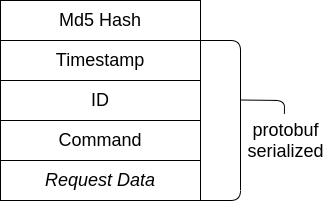
\includegraphics[width=.5\textwidth]{figures/methodology/methodology-request-message}%
	}
	\subfloat[]{%
		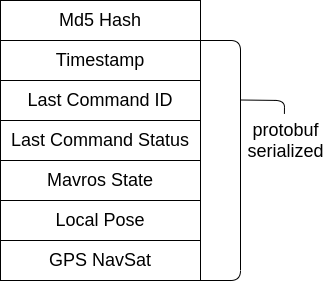
\includegraphics[width=.5\textwidth]{figures/methodology/methodology-response-message}
	}
	
	\label{fig:control-messages}
\end{figure}

HEART\_BEAT will have command id 0. SET\_OFFBOARD, SET\_RETURN\_TO\_HOME, SET\_ARM, and GOTO will have incremental id. That is for every new command, the id will increment by one. HEART\_BEAT reply will have the last command id received by pegasus\_commander and the status of its execution. Last command status is set to true when the command has been executed. Figure~\ref{fig:communitation-controller-commander} illustrates the communication between one pegasus\_controller and two pegasus\_commander.

\begin{figure}
	\centering
	\caption[Communication between \texttt{pegasus\_controller} and two \texttt{pegasus\_commander}.]{\small GOTO command communication diagram between \texttt{pegasus\_controller} and two \texttt{pegasus\_commander}.}
	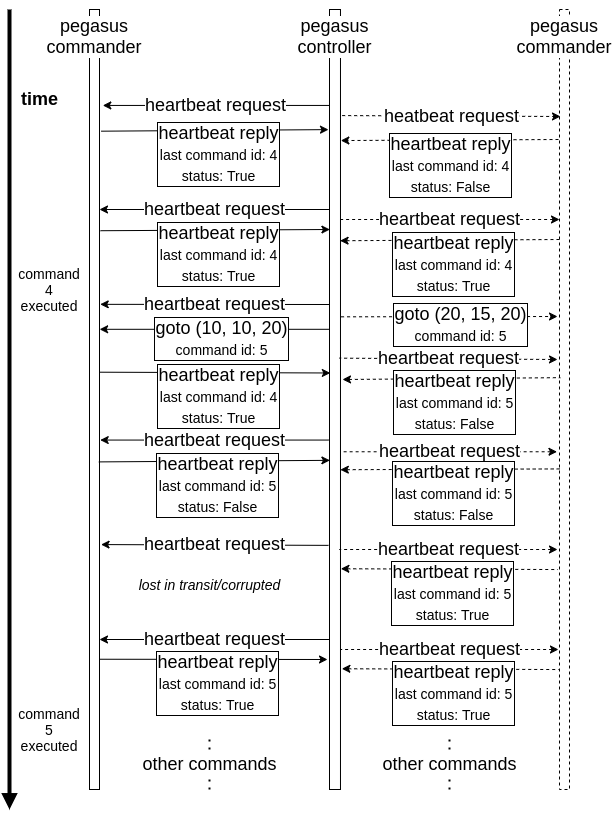
\includegraphics[width=5in]{figures/methodology/methodology-commander-controller-communication}
	\label{fig:communitation-controller-commander}
\end{figure}

\subsubsection{Pegasus\_controller}

Pegasus\_controller will be responsible for:
\begin{itemize}
	\item Calculating and maintaining the transformations between the local map frames of each drone and the global map frame.
	\item Coordinating and sending control messages to the drones.
	\item Monitoring the link with the drones by sending heart beat control message.
	\item Publishing local pose, global GPS coordinates and state of each drone, received in the heart beat reply as ROS topics.
	\item Calling image acquisition service to acquire images from the drones.
\end{itemize}

\begin{figure}
	\centering
	\caption[Architecture of \texttt{pegasus\_controller}.]{\small Architecture of \texttt{pegasus\_controller}.}
	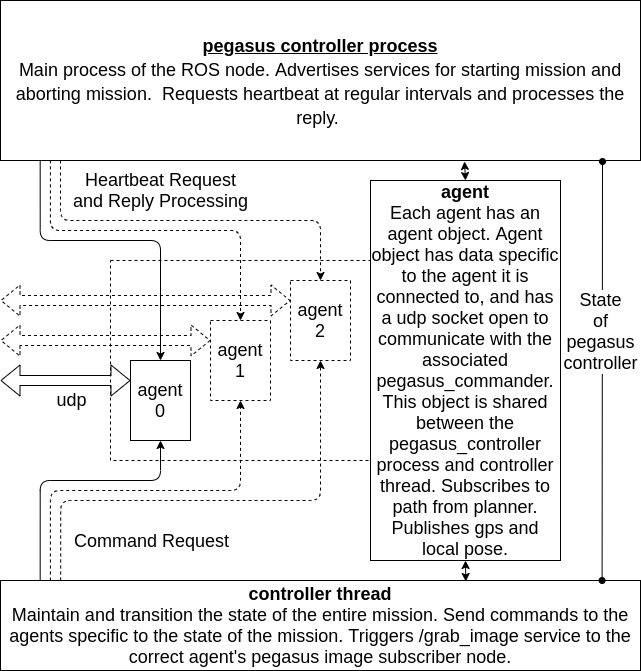
\includegraphics[width=5in]{figures/methodology/methodology-pegasus-controller}
	\label{fig:pegasus-controller}
\end{figure}

The architecture diagram of pegasus\_controller is given in Figure~\ref{fig:pegasus-controller}.
\begin{figure}
	\centering
	\caption[State diagram of \texttt{pegasus\_controller}.]{\small State diagram of \texttt{pegasus\_controller}.}
	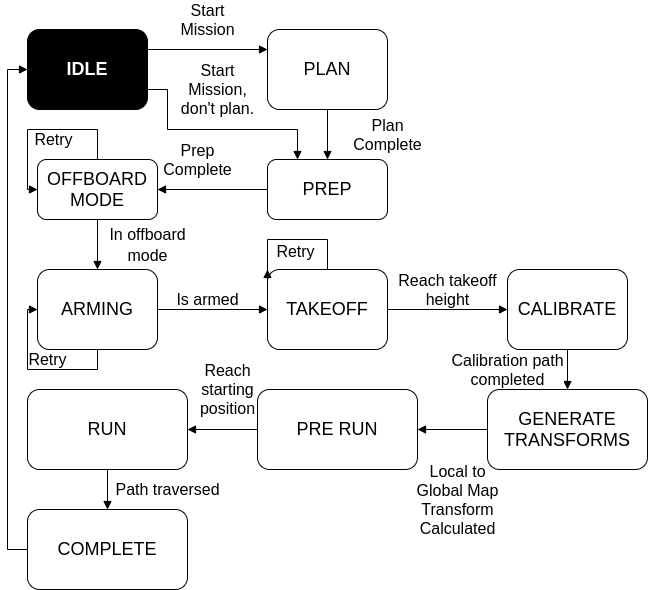
\includegraphics[width=5in]{figures/methodology/methodology-controller-state-diagram}
	\label{fig:controller-state-diagram}
\end{figure}

The state diagram in Figure~\ref{fig:controller-state-diagram} can be further elaborated as follows:
\begin{itemize}
	\item \textit{IDLE.} It will not do anything.
	\item \textit{PLAN.} Call services provided by pegasus\_planner. 
	\item \textit{PREP.} Prepare the drone to enter offboard mode.
	\item \textit{OFFBOARD\_MODE.} It will send SET\_OFFBOARD control message to the drones and wait for confirmation.
	\item \textit{ARMING.} It will send SET\_ARM control message to the drones and wait for confirmation.
	\item \textit{TAKE\_OFF.} It will takeoff drones to operational height.
	\item \textit{CALIBRATE.} It will send the calibration path to the drones and coordinate the flight of the drone along the calibration path and capture the corresponding local poses and global GPS positions for calculation the map transformations.
	\item \textit{GENERATE\_TRANSFORMS.} It will generate the transforms between the local map frame of each drone and the global map frame using the corresponding points collected in CALIBRATE state.
	\item \textit{PRE\_RUN.} Move the drones to starting position.
	\item \textit{RUN.} It will execute path of the drones in a coordinated manner.
	\item \textit{COMPLETE.} It will reach this state when the system's execution is complete. Set the drone to Return mode by sending SET\_RETURN\_TO\_HOME control message.
\end{itemize}

The drone will takeoff in its home position. After it reaches its operational height, it will follow a predefined routine from CALIBRATE state to PRE\_RUN state as shown in Figure~\ref{fig:calibration-routine}.  All the drones will be positioned at the origin of the global map (pegasus\_map) at different altitudes in PRE\_RUN state. For a mission with operational height $z_o$ and $n$ drones, the $i^{th}$ drone, were $0 <= i < n$ will have $z = z_o + i * 2$ meters altitude in PRE\_RUN state. 

\begin{figure}
	\centering
	\caption[Predefined routine before the start of the coordinated path traversal]{\small Predefined routine before the start of the coordinated path traversal. Steps 1-4 will be executed in CALIBRATE state, step 5 will be executed in PRE\_RUN state, and in step 6 the drone will move to the first pose in the planned path.} 
	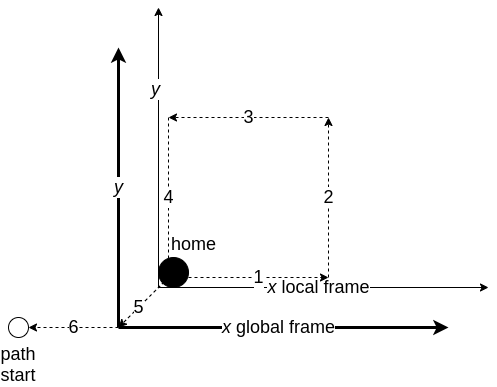
\includegraphics[width=5in]{figures/methodology/methodology-calibration-routine}
	\label{fig:calibration-routine}
\end{figure}

In GENERATE\_TRANSFORM state , algorithm~\ref{alg:find-transforms} will be used to find transforms between local map of each drone and the global map. The problem of finding transforms between all the local and global maps can be done with planar homography because the z axis of all the maps are parallel and pointing upwards.

In RUN state,pegasus\_commander will be configurable to allow two types of movement:
\begin{itemize}
	\item \textit{Towards.} The drones will face toward the direction it is moving. During image acquisition the drones will orient itself by setting their yaw to 0\degree as shown in Figure~\ref{fig:towards-movement}.
	\item \textit{Strafe.} The drones will always have its yaw at 0\degree. They will move sideways to the next viewpoint. This movement requires less time when the viewpoints are separated by small distances. Figure~\ref{fig:strafe-movement} shows this movement.
\end{itemize}

\begin{figure}
	\centering
	\caption[Movement types for drones.]{\small 
		Drones will be able to be configured to follow either (a) Towards movement, or  (b) Strafe movement. Towards movement takes more time than strafe movement because it has to know whether it has reached the destination pose in step 5, and if it has properly aligned to take image in step 6. In strafe movement the drone is already aligned to take image and it just needs to know wheather it has reached the destination pose in step 4. }
	\subfloat[]{%
		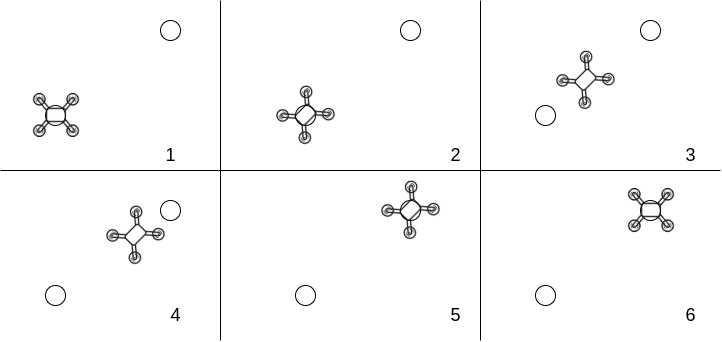
\includegraphics[width=5in]{figures/methodology/methodology-towards-movement}%
		\label{fig:towards-movement}
	}
	
	
	\subfloat[]{%
		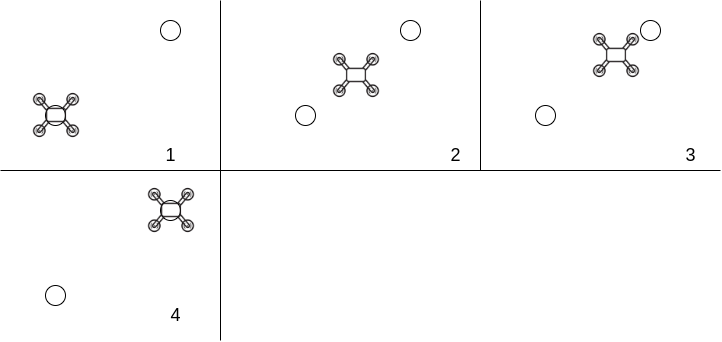
\includegraphics[width=5in]{figures/methodology/methodology-strife-movement}
		\label{fig:strafe-movement}
	}
	\label{fig:movement-types}
\end{figure}

Image acquisition will be skipped if the drone has already visited the viewpoint to avoid duplicate images.

\renewcommand{\algorithmicrequire}{\textbf{Input:}}
\renewcommand{\algorithmicensure}{\textbf{Output:}}
\renewcommand{\algorithmicforall}{\textbf{for each}}
\begin{algorithm}
	\caption{Find Local To Global Transformation}
	\label{alg:find-transforms}
	\begin{algorithmic}
		\REQUIRE $L$: set of all corresponding local poses
		\REQUIRE $G$: set of all corresponding global GPS positions
		\REQUIRE $O$: global map origin GPS coordinate
		\ENSURE $T$: transformation between local and global map
		\STATE $\widetilde{O} \gets \textsc{Convert-to-UTM}(O)$
		\STATE $\widetilde{G} \gets \textsc{Convert-to-UTM}(G)$
		\STATE $M \gets \widetilde{G} - \widetilde{O}$
		\STATE $\widehat{M} \gets \textsc{Remove-Z-axis}(\widetilde{M})$
		\STATE $\widehat{L} \gets \textsc{Remove-Z-axis}(L)$
		\STATE $H \gets \textsc{Find-Homography}(\widehat{L}, \widehat{M}, \text{RANSAC})$
		\STATE $T \gets \begin{bmatrix}
		H_{1,1} & H_{2,1} & 0 & H_{3,1} \\
		H_{1,2} & H_{2,2} & 0 & H_{3,2} \\
		0 & 0 & 1 & 0 \\
		0 & 0 & 0 & 1
		\end{bmatrix}$
		
	\end{algorithmic}
\end{algorithm}

In COMPLETE state, the drones will return to their home position following the behavior defined in PX4 firmware. PX4 firmware ascends the drone to a safe altitude before returning them to home. To avoid collision, the drones' safe altitude should be set different from each other.

\subsubsection{Pegasus\_commander} \label{section:pegasus-commander}

Pegasus\_commander is a new ROS node, customized for this study that will use the topics and services provided by mavros to control the drone in off-board mode. It will receive control messages from the pegasus\_controller. It will also monitor the link between GCS and the drone, and if a HEART\_BEAT control message is not received for a particular duration, then the flight controller will be set to Return mode. The architecture diagram of this module is shown in Figure~\ref{fig:pegasus-commander}.
It will only respond to HEART\_BEAT control message with:
\begin{itemize}
	\item The last command id it received and the status of the command,
	\item State of mavros,
	\item Local Pose of the drone in the local map,
	\item GPS coordinates of the drone.
\end{itemize}

For SET\_ARM, SET\_OFFBOARD and SET\_RETURN\_TO\_HOME it calls the relevant mavros services. For GOTO, it publishes the pose it received to mavros until it reaches the desired pose. Algorithem ~\ref{alg:is-at-position} will be used to determine if the drone has reached the desired pose.

\renewcommand{\algorithmicrequire}{\textbf{Input:}}
\renewcommand{\algorithmicensure}{\textbf{Output:}}
\renewcommand{\algorithmicforall}{\textbf{for each}}
\begin{algorithm}
	\caption{Is at position.}
	\label{alg:is-at-position}
	\begin{algorithmic}
		\REQUIRE $P_e$: expected pose 
		\REQUIRE $P_a$: actual pose
		\REQUIRE $d$: offset distance
		\REQUIRE $y$: offset yaw
		\ENSURE $A$: Boolean True or False 
		\STATE $D \gets |\textsc{euclidean\_distance}(P_e.position, P_a.position)|$
		\STATE $Y_e \gets \textsc{get\_yaw\_from\_quaternion}(P_e.orientation) $
		\STATE $Y_a \gets \textsc{get\_yaw\_from\_quaternion}(P_a.orientation) $
		\STATE $Y \gets |Y_e - Y_a|$
		\STATE $A \gets (D < d) \land (Y < y)$
	\end{algorithmic}
\end{algorithm}

\begin{figure}
	\centering
	\caption[Architecture diagram of\texttt{ pegasus\_commander}.]{\small Architecture diagram of \texttt{pegasus\_commander}.} 
	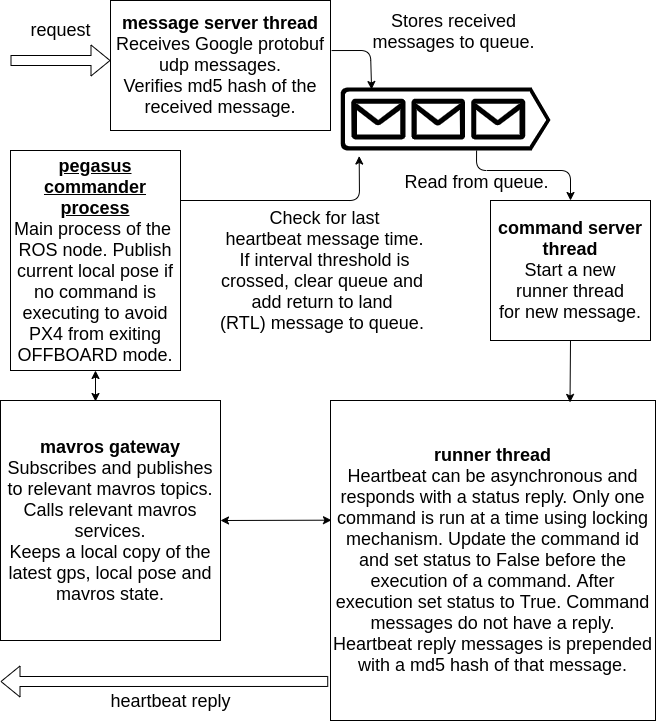
\includegraphics[width=5in]{figures/methodology/methodology-pegasus-commander}
	\label{fig:pegasus-commander}
\end{figure}

\subsubsection{PX4}
The drone runs PX4 Firmware on the flight controller. The flight controller's movement and altitude can be controlled in Offboard mode through the MAVlink protocol. This mode supports only a very limited set of MAVLink commands.

MAVLink commands supported in Offboard modes are:
\begin{itemize}
	\item SET\_POSITION\_TARGET\_LOCAL\_NED: Control vehicle position.
	\item SET\_ATTITUDE\_TARGET: Control vehicle altitude and orientation.
\end{itemize}

PX4 supports the coordinate frames (coordinate\_frame field): MAV\_FRAME\_LOCAL\_NED and MAV\_FRAME\_BODY\_NED.

A stream of setpoint commands must be received by the vehicle prior to engaging the mode, and in order to remain in the mode (if the message rate falls below 2Hz the vehicle will stop). In order to hold position while in this mode, the vehicle must receive a stream of setpoints for the current position.

Offboard mode requires an active connection to a remote MAVLink system (e.g. companion computer or GCS). If the connection is lost, after a timeout (COM\_OF\_LOSS\_T) the vehicle will attempt to land or perform some other failsafe action. The action is defined in the parameters COM\_OBL\_ACT and COM\_OBL\_RC\_ACT which can be set through mavros' mavparam.

\subsubsection{Mavros}

Mavros is a ROS node that provides ROS interfaces for communication with various autopilots with MAVLink communication protocol.
The ROS services provided by Mavros,  of interest for this system are:
\begin{itemize}
	\item \textit{mavros/set\_mode.} Required to set mode of the flight controller to off-board mode and return to launch mode.
	\item \textit{mavros/cmd/arming.} Required to arm the flight controller.
\end{itemize}

The ROS topics published by Mavros, useful for this system are:
\begin{itemize}
	\item \textit{mavros/state.} Publishes the state of the flight controller.
	\item \textit{mavros/local\_position/pose.} Publishes pose, i.e. position and orientation of the flight controller in the local frame. Mavros handles the translation between NED and ENU conventions.
	\item \textit{mavros/global\_position/global.} Publishes the GPS coordinates, i.e. latitude, longitude and altitude of the flight controller.
\end{itemize}

The ROS topics subscribed by Mavros, that this system will use are:
\begin{itemize}
	\item \textit{mavros/setpoint\_position/local.} Set the pose, i.e. position and orientation that the flight controller is desired to achieve in local frame.
\end{itemize}


\subsection{Image Acquisition}

This layer provides image acquisition service. The GCS will be able to request geo-tagged image from the drone in flight, using image acquisition service. The software components in this layer are gscam and pegasus\_image\_publisher in the drones and pegasus\_image\_subscriber in the GCS. The gscam ROS node is used to publish camera video feed as ROS camera topic using gstreamer. Mavros is used to acquire GPS location of the image captured. The pegasus\_image\_subscriber will provide a ROS service in the GCS which is called by pegasus\_controller to acquire images at the viewpoints. The pegasus\_image\_subscriber will be a udp client that requests image from the pegasus\_image\_publisher udp server in the drone. For multiple drones there will be multiple pegasus\_image\_subscriber running under different ROS namespace in the GCS. The subscriber and the publisher will transfer data with each other using the packet as shown in Figure~\ref{fig:image-packet}.

\begin{figure}
	\centering
	\caption[Packet structure for image acquisition.]{\small Packet structure for image acquisition.} 
	\label{fig:image-packet}
	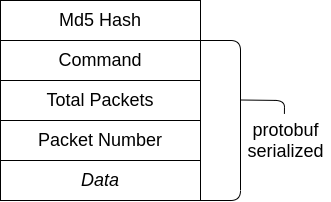
\includegraphics[width=3in]{figures/methodology/methodology-Image-packet}
\end{figure}

The same packet structure will be used by both the subscriber and publisher, however the commands are different for each:
\begin{itemize}
	\item \textit{REQUEST.} This request will be sent from subscriber to the publisher. The publisher will drop the previous buffer, capture a new image, add GPS tag to it, segment the image into multiple packets and store in buffer.
	\item \textit{REPLY.} The publisher will respond to the subscriber for the REQUEST packet. It will have the total packets in the buffer for the image requested.
	\item \textit{PKT.} The subscriber will request image packets from the publisher using the packet number it wants. It will request the same packet number until it receives the packet and then increment the packet number. The publisher will fill the data section with the image data and reply. The request will be made till the packet number reaches the total packets received in REPLY.
	\item \textit{ERR.} If the publisher cannot find the packet number the subscriber is requesting for, it will respond with ERR message.
\end{itemize}

The communication diagram is illustrated in Figure~\ref{fig:image-communication-diagram}.

\begin{figure}
	\centering
	\caption[Communication diagram for image acquisition.]{\small Communication diagram for image acquisition.} 
	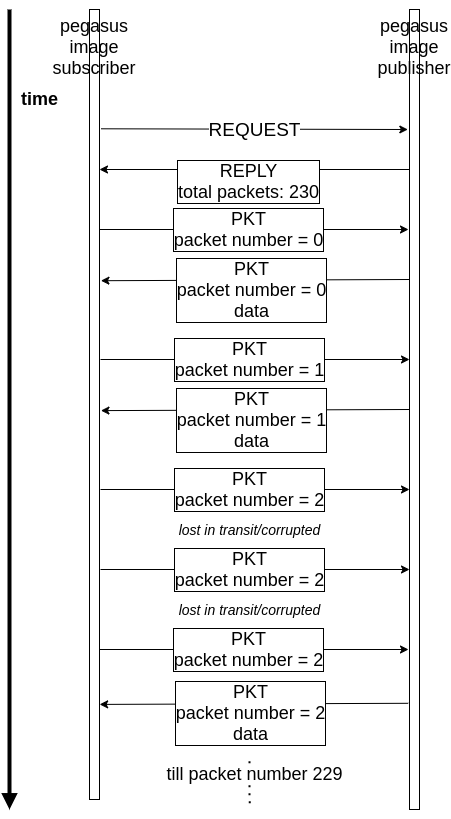
\includegraphics[width=4in]{figures/methodology/methodology-image-communication-diagram}
	\label{fig:image-communication-diagram}
\end{figure}


\subsubsection{Pegasus\_image\_publisher}

The gscam ROS node will provide the USB camera video feed as ROS topic. The pegasus\_image\_publisher node will subscribe to the ROS camera topic and GPS topic published by mavros. When it receives a REQUEST message from the pegasus\_image\_subscriber, it will get the current video frame and gps data, and store GPS data using Exchangeable Image File (EXIF) format. It will store the geo-tagged image in buffer till a new REQUEST message is received. It will provide image data to the subscriber from the current buffer.


\subsubsection{Pegasus\_image\_subscriber}

The pegasus\_image\_subscriber will provide image acquisition service to the GCS. It will expose ROS service \textit{/[drone\_namespace]/grab\_image}. For multiple drones there should be multiple pegasus\_image\_subscriber running under different ROS namespace in the GCS. It will receive the image and store it in the local directory under the name \textit{[drone-namespace]-i.jpeg}. Where \textit{i} is the image number.

\subsection{Map Building}
This layer will build the map from the images captured during the mission. This will be run after the drones have finished their mission. This layer has two components, pegasus\_image\_rectify and WebODM.

\subsubsection{Pegasus\_image\_rectify}
Pegasus\_image\_rectify will use the camera calibration file generated by camera\_calibration node available in image\_pipeline ROS package to rectify the images received from the drones. The images capture from the drones will follow the naming convention of \textit{[drone-namespace]-i.jpeg}. The pegasus\_image\_rectify will only process the images for the associated camera calibration file by identifying the images using the drone-namespace. It will also provide a feature to select region of interest to crop the image received from the drones. The rectified images are saved with the same filename in another output directory in the GCS.

\subsubsection{WebODM}
WebODM provides a web based GUI to use Open Drone Map (ODM). The operator will upload the rectified images to WebODM and generate orthographic map, and 3D point cloud among other features provides by ODM.
\begin{figure}
	\centering
	\caption[WebODM]{\small WebODM application for generating map from images.} 
	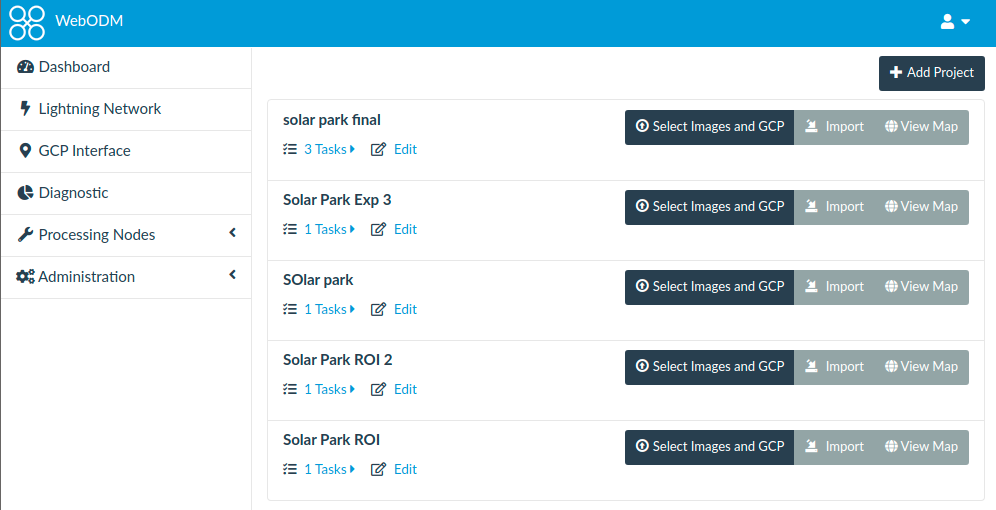
\includegraphics[width=6in]{figures/methodology/webodm}
	\label{fig:webodm}
\end{figure}

\subsection{Pegasus\_fov}
Pegasus\_fov will be a helper node to assist the operator in selecting a good grid size for the viewpoints. It will calculate the area covered by an image given the operational height of the drone and the camera calibration file. Camera calibration file has:

\begin{itemize}
	\item $w$. Image width.
	\item $h$. Image height.
	\item $K$. Camera matrix, where 
	$$K = \begin{bmatrix}
	f_x && s   && x_0 \\
	0   && f_y && y_0 \\
	0   && 0   && 1
	\end{bmatrix}$$
\end{itemize}

$f_x$ and $f_y$ are $x$ and $y$ focal length. $x_0$ and $y_0$ are principal point offset. $s$ is the axis skew.

To find the angle of view,
$$ \theta_x = 2 \times \tan^{-1}(\frac{w}{2 \times f_x}) $$

$$ \theta_y = 2 \times \tan^{-1}(\frac{h}{2 \times f_y}) $$

From $\theta_x$ and $\theta_y$, the area of coverage per viewpoint from altitute $z$ can be calculated.

$$ x = 2 \times \tan(\frac{\theta_x}{2}) \times z $$
$$ y = 2 \times \tan(\frac{\theta_y}{2}) \times z $$ 

$(x, y)$ will be the area captured by the camera at altitude $z$. The operator can use this information to choose the size of the grids in path planning.

This node will be accessible using rosrun with parameters \_camera\_file and \_height as follows:

\begin{verbatim}
$ rosrun pegasus_uav_ros pegasus_fov.py 
    _camera_file:=$(pwd)/src/pegasus_uav_ros/calibration/mobius.yaml 
    _height:=20
\end{verbatim}

\section{Chapter Summary}
All chapters except Chapter 1 must include an introductory paragraph/s and a chapter summary.

\FloatBarrier